\documentclass[twoside,openright,% regular options
               DIV10,BCOR7mm,% page size options
               parskip=half,
               headings=small
               %,draft
               ]% KOMA options
               {scrbook} % Class: KOMA-script version of 'report'
    
\usepackage{Informe}

%%------------%%
%%            %%
%%    META    %%
%%            %%
%%------------%%
\author{Alvaro Alonso - Maximiliano Badaloni - Fernando Cladera}
\title{Proyecto Final de Estudios}

%%%%%%%%%%%%%%%%%%%%%%%%%%%%%%%%%%%%%%%%%%%%%%%%%%%%%%%%%%%%%%%%%%%%%%%%
%%----------------------%%
%%            		%%
%%    INICIO DOCUMENTO  %%
%%            		%%
%%----------------------%%
\begin{document}

\begin{titlepage}

\begin{center}

% Upper part of the page
%\includegraphics[width=0.15\textwidth]{./logo}\\[1cm]    

\textsc{\LARGE Universidad Nacional de Cuyo}\\[1.5cm]
\textsc{\LARGE Facultad de Ingeniería}\\[1.5cm]

\textsc{\Large Proyecto Final de Estudios}\\[0.5cm]
\textsc{\Large Ingeniería en Mecatrónica }\\[0.5cm]

% Title
\HRule \\[0.4cm]
{ \huge \bfseries Planta de Control de Nivel:

Diseño, construcción y programación}\\[0.4cm]

\HRule \\[1.5cm]

% Author and supervisor
\begin{minipage}{0.4\textwidth}
\begin{flushleft} \large
\emph{Autores:}\\
Alvaro \textsc{Alonso} \\
Maximiliano \textsc{Badaloni} \\
Fernando \textsc{Cladera Ojeda}
\end{flushleft}
\end{minipage}
\begin{minipage}{0.4\textwidth}
\begin{flushright} \large
\emph{Director:} \\
Prof. Mg. Ing. Alfredo Ernesto \textsc{Puglesi}
\end{flushright}
\end{minipage}

\vfill

\begin{minipage}[c]{0.9\textwidth}
  \centering
  %\hfill
  
\includegraphics[height=20mm]{Caratula/Logos/LogoFacu.pdf}
\end{minipage}

\vspace{1cm}

% Bottom of the page
{\large \today}

\end{center}

\end{titlepage}

%\chapter*{Glossaire}
%\addcontentsline{toc}{chapter}{Glossaire}
%\markboth{Glossaire}{Glossaire}


% 
% \newglossaryentry{OFDM}{name=OFDM,description={Orthogonal Frequency Division Multiplexing}}

%%%%%%%%%%%%%%%%%%%%%%%%%%%%%%%%%%%%%%%%%%%%%%%%%%%%%%%%%%%

%% Acronyms

\newacronym{pwm}{PWM}{moduladores por ancho de pulsos}

\newacronym{adc}{ADC}{Conversor análogo digital}

\newacronym{gpio}{GPIO}{General Purpose Input/Output}

\newacronym{pid}{PID}{proporcional-integral-derivativo}

\newacronym{enib}{ENIB}{École Nationale d'ingénieurs de Brest}

%%%%%%%%%%%%%%%%%%%%%%%%%%%%%%%%%%%%%%%%%%%%%%%%%%%%%%%%%%%

%% Definitions

% Algunas palabras votan para pasar a ser definiciones!

%%%%%%%%%%%%%%%%%%%%%%%%%%%%%%%%%%%%%%%%%%%%%%%%%%%%%%%%%%%%%%%%%%%%%%%%
%%----------------------%%
%%            		%%
%%   	 INDICES	%%
%%            		%%
%%----------------------%%
\frontmatter

\tableofcontents
\listoffigures
%\listoftables
\markboth{}{}
\pagestyle{empty}
%\vspace{-2cm}
%---------------------------%

\chapter{Abstract}

Acá va el abstract

%%%%%%%%%%%%%%%%%%%%%%%%%%%%%%%%%%%%%%%%%%%%%%%%%%%%%%%%%%%%%%%%%%%%%%%%
%%-----------------------------%%
%%                             %%
%%  CAPÍTULOS PRINCIPALES      %%
%%                             %%
%%-----------------------------%%
\pagestyle{plain}
\mainmatter
\chapter{Introducción}
\label{ch:intro}
\section{Hello world}
El Gobierno yugoslavo partió al exilio a mediados de abril de 1941, cuando quedó clara la victoria de Alemania y de sus aliados del Eje en su campaña de castigo. 
El Gobierno acabó por instalarse en Londres y trató de representar al país —en la práctica desmembrado e inmerso en una guerra civil paralela a la guerra mundial— ante los Aliados. 
Víctima de sus disputas internas y de su incapacidad para controlar los acontecimientos en Yugoslavia, fue finalmente forzado a alcanzar un acuerdo en desventaja con Tito que supuso su desaparición. 
Fue sustituido por un Gobierno de coalición controlado en la práctica por los comunistas yugoslavos.

\begin{align}
	\frac{1}{\sqrt{\lambda}} &= -2 \log_{10} {\left ( \frac{k/D}{3,7} + \frac{2,51}{Re \sqrt{\lambda}} \right )}
\end{align}
\chapter{Diseño y Ensamblado}
\label{ch:DisenoEnsamblado}

En esta sección se describirán los pasos necesarios para la concreción física
del proyecto.
Se comenzará con la confección e interpretación del diagrama de cañerías e
instrumentación, con el objetivo de validar la solución propuesta en
\ref{sec:SolucionPropuesta}.
Luego se hará énfasis en la construcción de la planta a partir de los elementos
disponibles.
Se describirá en detalle cada uno de ellos y se hará mención de
las decisiones constructivas tomadas durante el ensamblado.

\section{P\&ID}
\label{sec:p&id}

\subsection{Diagrama de cañerías e instrumentación}
Un diagrama de cañerías e instrumentación es un esquema de la planta en donde
pueden observarse todos los elementos que componen el proceso.
Estos diagramas emplean símbolos para representar cada elemento y sus
conexiones.
Los elementos presentes en este esquema están regidos por la norma
\emph{Standard S5.1 Instrumentation Symbol Specification}.

El diagrama permite una rápida comprensión del proceso, y se denomina
corrientemente \gls{pyid}.

En los diagramas \gls{pyid} encontramas grafícados los elementos 
como un círculo, cada uno de ellos debe ir acompañado de una denominación,
que utiliza la siguiente codificación:

\begin{itemize}  
 \item \textbf{Primer letra:}
 designa la variable medida. Puede ser :
 \begin{itemize}
  \item Presión
  \item Nivel
  \item Caudal
  \item Temperatura
 \end{itemize}

 \item \textbf{Letras siguientes:}
 designa la función del componente, o modifica el sentido de la primer letra.
 Puede ser:
 \begin{itemize}
  \item Indicador
  \item Almacenaje de datos
  \item Controlador
  \item Transmisor
  \item Alarma
 \end{itemize}
\end{itemize}

Al mismo tiempo estos círculos pueden estar intersectados por una linea la cual 
indica su ubicación:

\begin{itemize}
 \item Sin línea: En el campo
 \item Continua: En la sala de control
 \item Trazos: Fuera del alcance del operario
\end{itemize}

Como su nombre lo indica también esta presente en el diagrama la descripción de las
cañerías que forman el sistema, esto incluye el material y los diámetros de las mismas.
Cabe destacar que en este diagrama y en esta instancia no es necesario especificar las 
longitudes y accesorios, dado que ello forma parte de un diagrama que se debe realizar 
en una etapa posterior del proyecto.

También se diferencia en el diagrama la naturaleza de cada señal, las cuales se describen
a continuación:

\begin{itemize}
 \item Tubería:
 Línea continua.
 \item Señal hidráulica:
 Línea continua intersectada con líneas perpendiculares en forma de L.
 \item Señal neumática:
 Linea continua intersectada por pequeñas líneas paralelas. 
 \item Señal eléctrica:
 Línea de trazos.
\end{itemize}


\subsection{P\&ID de nuestra planta}
De acuerdo a los componentes detallados en la Sec.
\ref{sec:MaterialesDisponibles} se realizó el esquema \gls{pyid} de la planta
de control de nivel.
Para la correcta comprensión de este capítulo es indispensable contar con el
esquema, que puede encontrarse en la Fig. \ref{img:pyid}.

\begin{figure}
	\centering
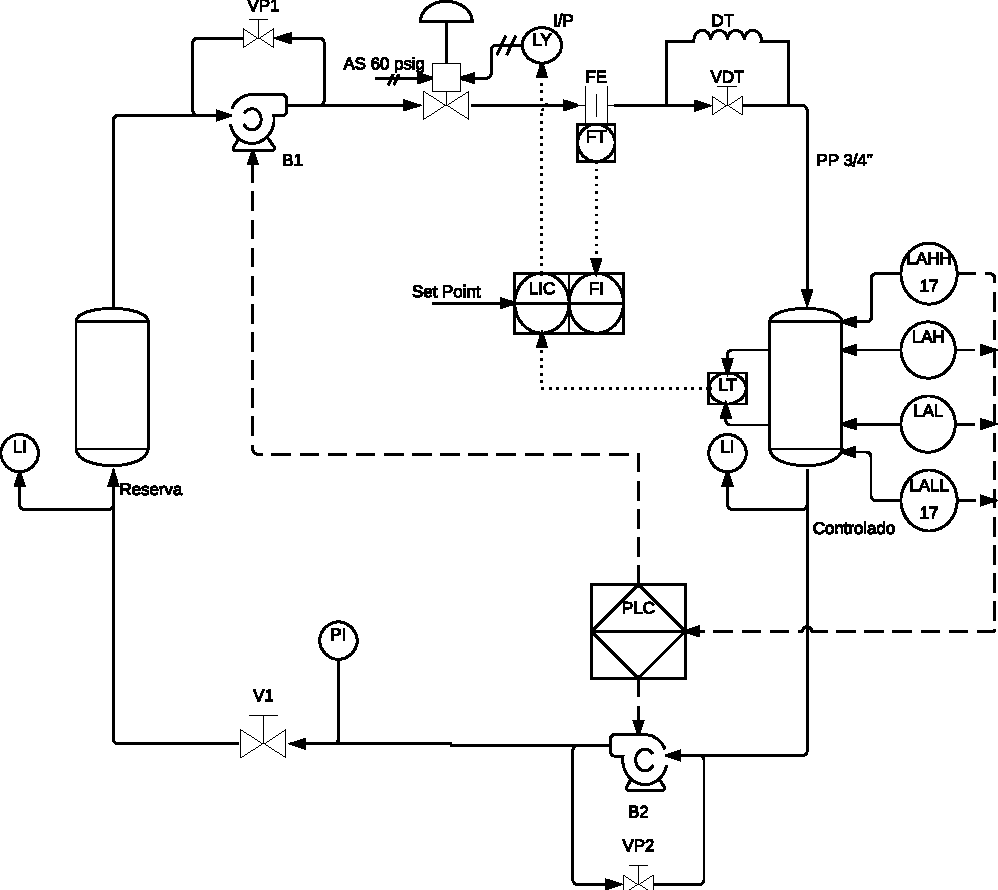
\includegraphics[width=\textwidth]{Cap2-DisenoEnsamblado/images/p&id.pdf}
	\caption{Diagrama P\&ID}
	\label{img:pyid}
\end{figure}

Las diferentes partes del diagrama se explicarán a continuación:

\subsubsection{Líneas}

\begin{itemize}
 \item Línea de trazos: 24 V
 \item Línea de puntos: 4 - 20 mA
 \item Línea continua: tubo de polipropileno de 3/4``
\end{itemize}

\subsubsection{Elementos}

En la Tab. \ref{tab:elementos}se presentan los elementos
que forman parte del diagrama \gls{pyid}. Se muestra en la misma
los simbolos que tienen cada una de las partes del sistema, así como
también se detalla el significado de las siglas que acompañan a
cada uno.

\begin{table}[H]
\small
\centering
\renewcommand*{\arraystretch}{0.3}

\begin{tabular}{*{2}{m{0.435\textwidth}}}
\hline
Tanque e indicador de nivel en tanque

LI: Level Indicator
  &\begin{center}
    %\rule{0.4\textwidth}{0.3\textwidth}
    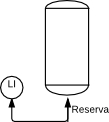
\includegraphics[height = 0.08\textwidth]
	{Cap2-DisenoEnsamblado/images/tanque.png}
  \end{center}\\
\hline
Bomba centrífuga
  &\begin{center}
    %\rule{0.4\textwidth}{0.3\textwidth}
    
\includegraphics[height = 0.05\textwidth]
	{Cap2-DisenoEnsamblado/images/bomba.png}
  \end{center}\\
\hline
Válvula neumática
  &\begin{center}
    %\rule{0.4\textwidth}{0.3\textwidth}
    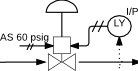
\includegraphics[height = 0.05\textwidth]
	{Cap2-DisenoEnsamblado/images/valvula.png}
  \end{center}\\
\hline
Placa orificio y DP Cell.

FT: Flow Transmitter
  &\begin{center}
    %\rule{0.4\textwidth}{0.3\textwidth}
    
\includegraphics[height = 0.05\textwidth]
	{Cap2-DisenoEnsamblado/images/placa.png}
  \end{center}\\
\hline
Tiempo muerto

DT: Death Time
  &\begin{center}
    %\rule{0.4\textwidth}{0.3\textwidth}
    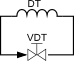
\includegraphics[height = 0.05\textwidth]
	{Cap2-DisenoEnsamblado/images/tmuerto.png}
  \end{center}\\
\hline
Controlador

LIC: Level Indicator and Controller
FI: Flow Indicator
  &\begin{center}
    %\rule{0.4\textwidth}{0.3\textwidth}
    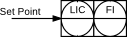
\includegraphics[height = 0.05\textwidth]
	{Cap2-DisenoEnsamblado/images/controlador.png}
  \end{center}\\
\hline
Transmisor e indicador de nivel

LI: Level Indicator
LT: Level Transmitter
  &\begin{center}
    %\rule{0.4\textwidth}{0.3\textwidth}
    
\includegraphics[height = 0.08\textwidth]
	{Cap2-DisenoEnsamblado/images/tnivel.png}
  \end{center}\\
\hline
Válvula e indicador de presión

PI: Pressure Indicator
  &\begin{center}
    %\rule{0.4\textwidth}{0.3\textwidth}
    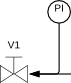
\includegraphics[height = 0.08\textwidth]
	{Cap2-DisenoEnsamblado/images/valvulam.png}
  \end{center}\\
\hline
\hline
\end{tabular}
\caption{Elementos del diagrama P\&ID}
\label{tab:elementos}
\end{table}

\subsubsection{Alarmas} 
\label{subsec:alarmas}

La gestión de alarmas se realiza a través del mismo sensor de nivel del sistema,
tomando entonces la información del mismo para detener el sistema en caso de pasar
los límites normales de trabajo. Este proceso se debería realizar mediante sensores
separados, pero debido al costo de los mismo se decidio obtener la información 
directamente desde el sensor de nivel del sistema.

En la Tab. \ref{tab:alarmas} se presenta la descripción de cada simbolo.

\begin{table}[H]
\small
\centering
\renewcommand*{\arraystretch}{0.3}

\begin{tabular}{*{2}{m{0.435\textwidth}}}
\hline
LAHH: Level Alarm High High
  &\begin{center}
    %\rule{0.4\textwidth}{0.3\textwidth}
    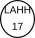
\includegraphics[height = 0.08\textwidth]
	{Cap2-DisenoEnsamblado/images/lahh.png}
  \end{center}\\
\hline
LAH: Level Alarm High
  &\begin{center}
    %\rule{0.4\textwidth}{0.3\textwidth}
    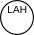
\includegraphics[height = 0.08\textwidth]
	{Cap2-DisenoEnsamblado/images/lah.png}
  \end{center}\\
\hline
LALL: Level Alarm Low Low
  &\begin{center}
    %\rule{0.4\textwidth}{0.3\textwidth}
    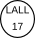
\includegraphics[height = 0.08\textwidth]
	{Cap2-DisenoEnsamblado/images/lall.png}
  \end{center}\\
\hline
LAL: Level Alarm Low
  &\begin{center}
    %\rule{0.4\textwidth}{0.3\textwidth}
    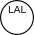
\includegraphics[height = 0.08\textwidth]
	{Cap2-DisenoEnsamblado/images/lal.png}
  \end{center}\\
\hline
PLC: Simbolo de la sección del programador encargado
de la gestión de alarmas
  &\begin{center}
    %\rule{0.4\textwidth}{0.3\textwidth}
    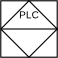
\includegraphics[height = 0.08\textwidth]
	{Cap2-DisenoEnsamblado/images/plc.png}
  \end{center}\\
\hline
\hline
\end{tabular}
\caption{Instalación del Driver Modbus}
\label{tab:alarmas}
\end{table}


\section{Estructura de Soporte}
\label{sec:EstructuraSoporte}

Dado que el objetivo principal del proyecto es que la planta sirva para fines
educativos, se opta por utilizar una estructura móvil.
De esta manera, la posición de la planta puede modificarse según se requiera.

\todo{imagen de la estructura}
La estructura, de caño estructural, puede apreciarse en la figura x.
Está dotada de cuatro ruedas con frenos de seguridad, que permiten fijar la
planta al momento de una demostración.
Sus dimensiones se presentan en la Tab. \ref{tab:dimensionesEstructura}.

\begin{table}
\centering
\begin{tabular}{|l|l|}
\hline
Alto & $1.55\,m$ (incluido ruedas)\\
Ancho &  $1.50\,m$\\
Profundidad &  $0.52\,m$\\
\hline
\end{tabular}
\caption{Dimensiones de la estructura de soporte}
\label{tab:dimensionesEstructura}
\end{table}
 
La estructura presenta en su sección media barras de refuerzo.
Sobre ellas se colocaron los tanques.
Además, sobre las barras se fijó una base de madera, donde se coloca la
válvula electroneumática, las celdas de presión diferencial
y las bombas.
La manguera que corresponde al tiempo muerto se colocó bajo
las barras de refuerzo.
En la parte superior de la planta se instaló una pequeña base de
madera donde irá montado el receptor inalámbrico.
Ya está incluida en la estructura el tablero, donde se
montarán los elementos eléctricos y electrónicos.
Sus dimensiones se observan en la Tab. \ref{tab:dimensionesTablero}.

\begin{table}
\centering
\begin{tabular}{|l|l|}
\hline
Alto & $62\,cm$\\
Ancho &  $30\,cm$\\
Profundidad &  $20\,cm$\\
\hline
\end{tabular}
\caption{Dimensiones del tablero.}
\label{tab:dimensionesTablero}
\end{table}

Al comienzo del proyecto la estructura de caño estaba ya soldada y pintada, con
las ruedas colocadas.
No obstante, el grupo de trabajo tuvo que barnizar las maderas.

\section{Cañerías}
\label{sec:Canerias}

\subsection{Mangueras y Caños}
Luego de analizar el esquema \gls{pyid}, se observa que las cañerías deben
formar un circuito cerrado (\emph{loop}), diferenciando
claramente las cañerías de vaciado y llenado.
Las conexiones fueron echas mayormente en caño de polipropileno de 3/4
pulgadas (presión de servicio: $11.7\,kgf/cm^2$ a $20^\circ C$).
En otros puntos del circuito, se optó por utilizar manguera de alta presión
telada de 3/4 pulgadas (presión de servicio: $10\,kgf/cm^2$ a $20^\circ C$).
Las cañerías utilizadas son suficientes para las presiones de trabajo del
proyecto, del orden de $1.2\,kgf/cm^2$.

Teniendo los elementos montados sobre la planta (bombas, tanques, válvula
electroneumática) se decidió la manera de realizar el conexionado.
El caño rígido presenta la dificultad de no tener tolerancia al momento de
realizar uniones.
Además, para realizar tuberías complejas con muchas curvas, es necesario
colocar un gran número de componentes suplementarios (uniones dobles,
niples).
La cañería se torna compleja, dificultando la comprensión del circuito
hidráulico por parte del alumno.
Es por ello que se opto por usar en diferentes partes de la planta mangueras
flexibles:

\begin{itemize}
  \item \textbf{Salida del tanque de reserva - entrada a la bomba B1}:
  se utilizo manguera flexible dado que la estructura no permitía colocar caños
  rígidos: los elementos de polipropileno necesarios eran más grandes que el
  espacio disponible en la estructura.

  \item \textbf{Salida de la bomba B1 - entrada a la válvula:}
  se utilizo manguera, para evitar una unión doble en un trayecto muy pequeño.
  
  \item \textbf{Salida de la válvula - entrada al tanque controlado:}
  debido a la longitud del tramo se opto usar caños rígidos.
  Además, se montaron los elementos de medición sobre la cañería (manómetro y
  placa orificio).
  
  \item \textbf{Salida del tanque controlado - entrada a la bomba B2:}
  debido al mismo problema de falta de espacio, se opto por el uso de manguera
  flexible.
  
  \item \textbf{Salida de la bomba - entrada al tanque de reserva:}
  esta conexión es la más larga y en ella van montados manómetros y
  válvulas manuales. Por ello, se eligió una cañería rígida de polipropileno.

  \item \textbf{Conexión de perturbación de las bombas:}
  se utilizó manguera flexible, para evitar uniones dobles y
  niples que requieren de una gran precisión durante el montaje.
 \end{itemize}

Por ultimo se procedió a pintar los caños mediante un código de colores.
 \begin{itemize}
  \item {\color{Cerulean} \textbf{Celeste:}} llenado del tanque controlado.
  \item {\color{YellowOrange} \textbf{Amarillo:}} vaciado del tanque controlado.
 \end{itemize}
El código de colores, si bien no es estándar en la industria, permite una fácil
comprensión del circuito hidráulico.
\todo{bella imagen de los colores de la cañería}

\subsection{Tiempo Muerto}
\label{subsec:tiempoMuerto}
Se colocó en la planta un circuito de tiempo muerto, que consta de 20 metros de
manguera negra de 1/2 pulgada.
El tiempo muerto se coloca en paralelo de la cañería de llenado (ver
\gls{pyid}).
Mediante una válvula manual puede elegirse utilizar o no el tiempo muerto.

El objetivo del tiempo muerto es alejar la acción de control del tanque
controlado.
El sensor de nivel tardará un tiempo adicional $t_d$ en observar los cambios
que se producen en la válvula electroneumática \cite{bib:ApuntesPuglesiTema2}.
La función de transferencia de la planta cambiará notablemente:
\begin{itemize}
 \item Por un lado, el retraso en la respuesta debe ser tenido en cuenta
 \begin{align}
  G_{td}(s) &= e^{-t_d\,s}\,G(s)
 \end{align}
 donde $G(s)$ corresponde a la función de transferencia de una planta sin
 tiempo muerto, y $G_{td}(s)$ es la misma planta con tiempo muerto.
  \item Por otro lado, se agregan pérdidas por rozamiento del
  fluido cambiando la función de transferencia original $G(s)$ de nuestra
  planta.
\end{itemize}
En conclusión, el proceso a controlar es diferente comparado con proceso sin
tiempo muerto.
La inclusión esta cañería adicional permite disponer de dos escenarios
diferentes para realizar prácticas, diseñando controladores distintos para
cada caso \cite{bib:ApuntesPuglesiTema2}.

\subsection{Válvulas manuales}

Diferentes válvulas manuales pueden encontrarse en las cañerías de la planta.
A continuación vamos a destacar la función de cada una de ellas:

\begin{itemize}
  \item \textbf{Desagote de los tanques:}
  para poder vaciarlos, se colocaron válvulas esféricas plásticas debajo de
cada tanque.

  \item \textbf{Control de caudal del tanque de reserva:} se colocó en serie
con la cañería de retorno. Se trata de una válvula manual, tipo exclusa.
  Esta válvula es importante ya que permite modificar el balance de masa y
ecualizar la planta.

  \item \textbf{Tiempo muerto:}
  tal como se describió en la Sec. \ref{subsec:tiempoMuerto}, esta válvula
esférica plástica permite activar la cañería de tiempo muerto.
  Notar en el \gls{pyid} que la válvula está sobre la cañería de llenado.
  Al cerrar la válvula, se fuerza el uso del tiempo muerto.
  Al abrirla, nada impide que el fluido circule por las dos cañerías al mismo
tiempo.
  No obstante, la pérdida de carga del tiempo muerto es significativamente
mayor que el de la cañería de llenado.
  Por ello, se considera que al abrir la válvula  el fluido sólo circula
por la cañería de llenado.

  \item \textbf{Perturbación de las bombas:}
  una válvula manual de tipo exclusa se coloca entre la tubería de aspiración y
la tubería de impulsión de las bombas.
  La apertura de esta válvula permitirá simular perturbaciones en las
bombas.
 Al abrir la válvula, el rendimiento de la bomba decae.
 \end{itemize}

\section{Tanques}
\label{sec:Tanques}

Los tanques almacenan el agua que del sistema, y las acciones de
control están dirigidas a establecer el nivel presente en los mismos.
Se ubicaron en los extremos, sobre las barras de refuerzo.
Se fijaron los tanques a las barras laterales de la estructura mediante
abrazaderas.

Son dos caños cloacales de $200\,mm$ de diámetro y un metro de altura, que
fueron
sellados en los extremos utilizando tapas.
La salida de agua hacia la tubería de aspiración de la bomba se realiza
mediante una conexión de tanque de 3/4 pulgada colocada en la base del tanque.
La entrada de agua se realiza por la parte superior, mediante un orificio
sencillo.

Además, en la base del tanque se colocó una segunda conexión de tanque de 3/4
pulgada, que se utilizará para medir el nivel.
Se conectan a esta cañería la celda de presión diferencial y una manguera
flexible transparente.
La manguera flexible, colocada en el lateral del tanque, permite obtener una
lectura visual directa del nivel.
Por otro lado, la celda de presión diferencial es un elemento de adquisición
que permite transformar un valor de presión (altura de la columna de agua) en
una señal $4$-$20\,mA$.
Se discutirá en la Sec. \ref{subsec:DPCell}.

Finalmente, dado que la cañería de aspiración de la bomba puede provocar
perturbaciones en la medición de la celda de presión diferencial, se optó por
colocar un niple en la conexión del tanque de aspiración.
De esta manera, se separan físicamente ambas cañerías, reduciendo las
perturbaciones en la medición de presión.
Cabe destacar que la inclusión del niple limita el nivel mínimo de la planta a
un 15\% del nivel total, aproximadamente.

\section{Bombas}
\label{sec:Bombas}

Se utilizaron en el proyecto dos bombas centrífugas, cuya función es
mantener en movimiento el agua en el sistema.
No se realiza ninguna acción de control sobre las
mismas, por lo que funcionarán de manera continua durante la operación de la
planta.

Las bombas centrífugas son máquinas hidráulicas, que absorben energía mecánica
de un motor y la restituyen en forma de energía hidráulica al fluido.
En las bombas centrífugas (o radiales), esta ganancia de energía se realiza por
medio de la fuerza centrífuga que imparten los álabes del rodete de la bomba.
Este tipo de bomba se caracteriza por entregar una presión elevada y un caudal
relativamente bajo \cite{bib:Mataix}.

Las especificaciones de las bombas utilizadas se presentan en la Tab.
\ref{tab:caractBombas}.

\begin{table}[t]
\centering
\begin{tabular}{|l|l|}
\hline
Marca & Czerweny\\
Caudal máximo &  $100\,l/min$\\
Altura máxima &  $12\,m = 1.2 kgf/cm^2$\\
Tensión & $220\,V$ monofásica $50\,Hz$\\
Corriente & $1.7\,A$\\
Seguridad & S1 IP44\\
\hline
\end{tabular}
\caption{Características de las electrobombas monofásicas}
\label{tab:caractBombas}
\end{table}

\subsection{Cavitación}
Para el ingreso del fluido a la bomba, es necesario realizar una succión
en la tubería de aspiración, descendiendo la presión del fluido.
Luego, la presión aumenta violentamente en el rodete de la bomba hasta alcanzar
la altura manométrica.
Debido a la baja presión en la tubería de aspiración, el fluido puede
evaporarse formando burbujas de vapor.
Luego, el rápido aumento de presión provoca una implosión de las burbujas.
Este fenómeno, conocido como \textbf{cavitación} genera ruido y disminuye la
vida útil de las las bombas \cite{bib:ApuntesMDFBombas}.

Para evitar la formación de burbujas de vapor, se opta por mantener la presión
en la tubería de aspiración lo más elevada posible.
Es por ello que las bombas se instalan en una posición baja.
Además, las bombas se colocaron lo más cerca posible de los respectivos
tanques disminuyendo las pérdidas en la cañería de aspiración.
Se fijaron mediante tornillos a la base de madera.

Durante la operación de la planta se observó un correcto funcionamiento de las
bombas, salvo cuando la perturbación se encuentra abierta: al incrementar la
velocidad en la tubería de aspiración, la presión desciende llegando hasta el
punto de vapor.

\section{Válvula Electroneumática}
\label{sec:ValvulaNeumatica}

En esta sección se hará énfasis en la válvula electroneumática.
Es un elemento central en nuestra planta, ya que es la encargada de efectuar
las acciones de control.

\subsection{Principio de funcionamiento}
\label{subsec:principioFuncionamiento}

\begin{figure}[ht]
        \centering
        \begin{subfigure}[b]{0.36\textwidth}
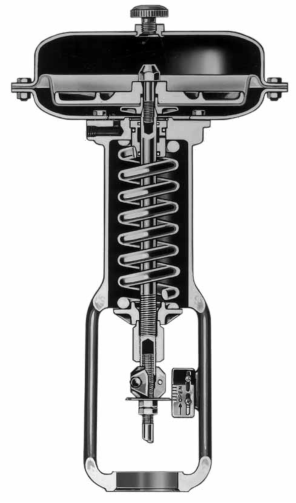
\includegraphics[width=\textwidth]
	{Cap2-DisenoEnsamblado/images/ActuadorValvNeum.pdf}
                \caption{Actuador neumático inverso.}
                \label{fig:actuadorValv}
        \end{subfigure}%
        ~
        \begin{subfigure}[b]{0.36\textwidth}
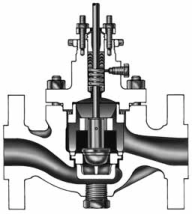
\includegraphics[width=\textwidth]{Cap2-DisenoEnsamblado/images/ValvGlob.pdf}
                \caption{Cuerpo de una válvula globo.}
                \label{fig:cuerpoValv}
        \end{subfigure}
        \caption{Elementos constitutivos de una válvula neumática.}
        \label{fig:elementosValv}
\end{figure}

Una válvula permite variar el caudal, dependiendo de la consigna que se
le envíe.
En las válvulas neumáticas, la consigna es un valor de presión de aire.
En la Fig. \ref{fig:elementosValv} se muestra un ejemplo de válvula de control
tipo globo, con actuador a diafragma inverso (aire para
abrir)\footnote{Figuras extraídas de \cite{bib:controlValveHandbook}.}.
La válvula está compuesta de dos elementos principales: el actuador
(Fig. \ref{fig:actuadorValv}) y el cuerpo de la válvula (Fig.
\ref{fig:cuerpoValv}).

El obturador en el cuerpo de la válvula (Fig. \ref{fig:cuerpoValv}) apoya
sobre un asiento.
La variación del caudal se produce gracias al orificio de paso variable
que forman al variar su posición relativa el conjunto asiento-obturador.
Sobre el vástago, encargado de modificar la posición del obturador,
actúan las fuerzas del actuador.
Como se observa en la Fig. \ref{fig:actuadorValv}, el actuador en una válvula
neumática es el conjunto diafragma-muelle.

Puede concluirse, a través del análisis de la válvula, que el caudal depende de
la presión de aire en el diafragma.
Generalmente, la presión oscila entre $3$ a $15\,psi$.
Esta presión de aire generalmente se obtiene mediante un convertidor
corriente-presión (I/P).
El convertidor toma en entrada una señal de corriente proveniente del \gls{plc}
($4$ - $20\,mA$) y lo transforma en un valor de presión para alimentar el
diafragma \cite{bib:ApuntesPuglesiValvulas}.
% \subsubsection{Rangeabilidad}
% Se denomina rangeabilidad a la razón entre el caudal máximo y el mínimo que
% puede controlar una válvula

\subsubsection{Tipos de obturador - Característica de caudal inherente}
Se denomina característica de caudal inherente a la variación del caudal de
la válvula en función de la carrera, manteniendo una presión diferencial
$\Delta p$ constante.
Para representar la característica inherente de una válvula, se grafica en
abscisas la carrera del obturador y en ordenadas el porcentaje de caudal máximo.

El conjunto asiento-obturador es la parte más importante de la válvula, ya que
es el elemento final que controla el caudal.
Dependiendo del tipo de conjunto asiento-obturador, se obtendrán distintas
características de caudal inherente.
Podemos distinguir tres conjuntos de válvula:
\begin{itemize}
  \item \textbf{Obturador Lineal:} el caudal es proporcional a la carrera
  \begin{align}
	q = k\,l
	\label{eq:inherenteLineal}
  \end{align}
  donde $q$ es el caudal a pérdida de carga constante, $k$ es una constante y
$l$ es la carrera del vástago.

  \item \textbf{Obturador Isoporcentual:}
  un incremento de carrera produce un cambio de caudal proporcional al caudal
que circulaba antes de la variación.
  \begin{align}
    \dfrac{dq}{dl} = a \, q
  \end{align}
  Operando, podemos reescribir esta expresión mediante una función exponencial.
\begin{align}
 q = b\,e^{a\,l}
 \label{eq:InherenteIsoporcentual1}
\end{align}
  donde $a$ y $b$ son constantes para una válvula dada.
  Si consideramos que
    \begin{align}
        l &= 0 \Rightarrow q = q_{min} = b\\
        l &= 1 \Rightarrow q = q_{max} = q_{min} \:e^a
    \end{align}
    podemos escribir la expresión \eqref{eq:InherenteIsoporcentual1} como
    \begin{align}
      \dfrac{q_{max}}{q_{min}} = e^a
    \end{align}
  \item \textbf{Obturador de apertura rápida:} permiten una brusca variación de
caudal con carreras pequeñas.
  No son utilizadas en el control regulatorio, ya que no permiten una
regulación fina del caudal.
\end{itemize}

En la Fig. \ref{fig:caractInherente}, se grafican las curvas de caudal
inherente para cada tipo de válvula.
A simple vista, la válvula con obturador lineal ofrece las mejores
características para el control regulatorio.
No obstante, como se expondrá posteriormente, las curvas características de las
válvulas quedan afectadas por el proceso en el que se utilizan.

\begin{figure}
 \centering
 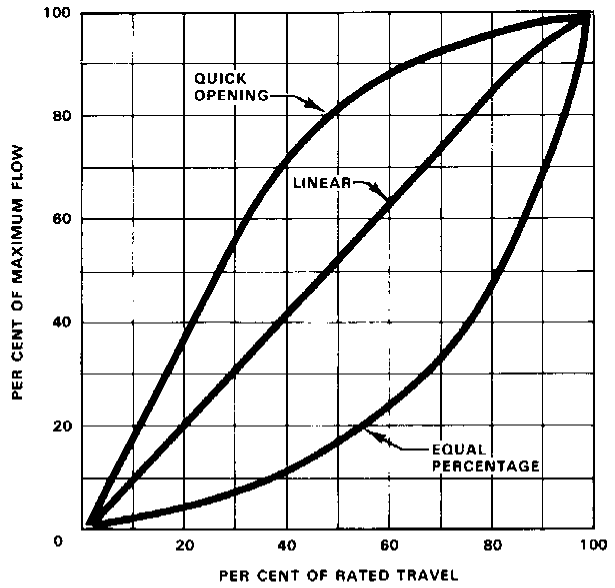
\includegraphics[scale=1.5]{Cap2-DisenoEnsamblado/images/Inherente.png}
 \caption{Características inherentes según el tipo de obturador.}
 \label{fig:caractInherente}
\end{figure}


\subsubsection{Característica de caudal efectivas}

La característica de caudal inherente se traza para una presión diferencial
$\Delta \,p$ constante.
No obstante, en un proceso real, $\Delta \,p$ no es constante.
En efecto, las pérdidas de carga y presión entregada por la bomba presentan
variaciones para diferentes caudales.

Se denomina característica de caudal efectiva a la variación del
caudal que atraviesa la válvula en función de su carrera, cuando la
válvula está inserta en una planta.
Dado que diferentes procesos proporcionarán distintos valores de  $\Delta
\,p$, la característica de caudal efectiva depende del proceso.
Evidentemente, esta curva se apartará de la característica de caudal inherente,
como se demostrará a continuación.

En una cañería, la presión que entregada por la bomba $H$ se utiliza para
vencer las pérdidas de carga en la cañería, contrapresiones y alturas
(reagrupadas en $H_2$) y en la válvula.
Denotando $\Delta \,p = H_1$
\begin{align}
 H &= H_1 + H_2
\end{align}
$H_2$ varía cuadráticamente con el caudal según la ley de \emph{Darcy-Weisbach}
\cite{bib:Franzini}
\begin{align}
 H_2  &= f \dfrac{L}{D^5}\dfrac{16\,Q^2}{2\,g\,\pi^2} + H_c
\end{align}
donde $L$ es la longitud equivalente de la cañería, $D$ es el diámetro y $H_c$
representa la altura piezométrica (contrapresiones y alturas).
$H$ varía siguiendo la curva característica caudal-presión de la bomba.

Se denomina coeficiente $r$ a la razón entre la pérdida de carga de la válvula
$H_1$ comparado con la pérdida de carga total del sistema.
\begin{align}
 r &= \dfrac{H_1}{H_1+H_2} = \dfrac{H_1}{H}
\end{align}
Evidentemente, $r = 1$ cuando la cañería no tiene pérdida de carga,
aproximándose la característica efectiva a la inherente.
Puede demostrarse \cite{bib:Creus} que
\begin{align}
 q_e &= \dfrac{1}{\sqrt{1-r+\dfrac{r}{{q_i}^2}}}
 \label{eq:coef_r_qe_qi}
\end{align}
siendo $q_e$ el caudal efectivo y $q_i$ el caudal inherente, que puede
obtenerse mediante las ecuaciones \eqref{eq:inherenteLineal} y
\eqref{eq:InherenteIsoporcentual1}.

Puede concluirse, a partir de la ecuación \eqref{eq:coef_r_qe_qi} que la curva
de caudal efectivo varía dependiendo de $H_2$.
Si se grafican las características efectivas de diferentes tipos de válvulas,
se observa que al disminuir $r$ (pérdida de carga elevada) una válvula
isoporcentual tiende a comportarse como una lineal,
y una válvula lineal se comporta como de apertura rápida.

Dado que las válvulas de apertura rápida no son utilizadas en el control
regulatorio, se escoge entre una válvula isoporcentual o lineal dependiendo de
la pérdida de carga de la planta, con el objetivo de tener una característica
efectiva ``lo más lineal posible''.

\subsection{Válvula utilizada en el proyecto}

En esta sección se describirá las características específicas de la válvula
utilizada en el proyecto, comparándolas con los principios de funcionamiento
descriptos en la Sec. \ref{subsec:principioFuncionamiento}.

\subsubsection{Especificaciones}
Se muestran en la Tab. \ref{tab:especifValvs} las especificaciones más
importantes de la válvula, consignada en su chapa de identificación.

\begin{table}
\centering
 \begin{tabular}{|c|c|}
  \hline
  Marca & Foxboro\\
  Modelo & V1S-30CNTSSEBK-50\\
	& Stabilflo Serie V1\\
 Actuador & P-50 EA-DO\\
 Medida Cuerpo & 3/4 roscado\\
 Interior & Globo vástago\\
 Característica $C_v$ & $=\%\,CV=10$\\
 Temperatura & $-30$ a $207^\circ C$\\
 Aire para & Abrir  \\
 Carrera & $19\,mm$ \\
  \hline
 \end{tabular}
 \caption{Especificaciones de la válvula electroneumática.}
 \label{tab:especifValvs}
\end{table}

\subsubsection{Electroposicionador}
Se especificó que la presión de aire en el diafragma varía entre $3\,psi$
(válvula cerrada) y $15\,psi$ (válvula abierta).
No obstante, en un convertidor I/P no hay una real comparación entre
la posición del vástago y la señal de corriente.
Ciertos fenómenos como la fricción en el vástago, perturbaciones del fluido,
fuerzas dinámicas, etc. pueden modificar la apertura de la válvula.

Para paliar estos problemas, la válvula incluye un electroposicionador Power
Genex.
Se trata de un controlador proporcional que compara la posición actual del
vástago con la consigna de corriente.
En caso de detectar errores, ejerce la acción de control correctiva para
asegurar la posición del vástago.

\begin{figure}[ht]
 \centering
 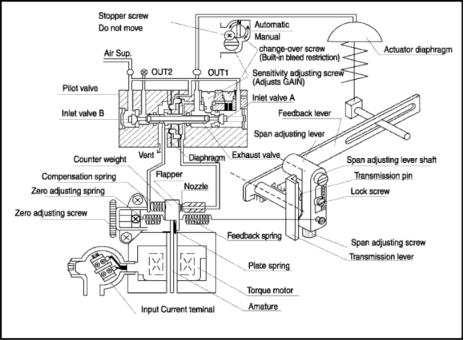
\includegraphics[scale=1.1]{Cap2-DisenoEnsamblado/images/PG-EPL.pdf}
 \caption{Esquema de funcionamiento, posicionador electroneumático.}
 \label{fig:elp-funcionamiento}
\end{figure}

En la Fig. \ref{fig:elp-funcionamiento} se muestra el esquema de
funcionamiento del electroposicionador.
La entrada de $4$-$20\,mA$ del controlador provoca una rotación en sentido
antihorario del motor de torque.
Lleva consigo al \emph{flapper}, liberando
presión por la boquilla (\emph{nozzle}) y moviendo la válvula hacia la
izquierda.
Se provoca un incremento de presión en \emph{OUT1} moviendo el diafragma del
actuador.

La varilla de feedback (\emph{feedback lever}) releva la posición del vástago y
la transmite mediante el resorte de feedback, que está vinculado con el
\emph{flapper}.
Se verifica que la posición del vástago de la válvula permanece constante
cuando el resorte de feedback iguala el par de rotación del motor de torque.
Otros elementos (\emph{compensation spring}, \emph{zero adjusting screw}) se
agregan para poder mejorar la estabilidad del bucle de control, como así
también poder calibrarlo\footnote{Explicación obtenida del manual del
electroposicionador.}.

La Tab. \ref{tab:especifElectroP} muestra las características más importantes
del electroposicionador presente en nuestra planta.

\begin{table}
 \centering
 \begin{tabular}{|c|c|}
  \hline
  Marca & Power Genex\\
  Modelo & EPL-FA15N4TL\\
  Señal entrada & $4$-$20\,mA$ DC\\
  Presión de entrada & $1.4$ - $7\,bar$ máximo\\
  Temperatura de trabajo & $-20$a $70^\circ$\\
  Seguridad & Ex dmb IIB+H2 T6 IP66\\
  \hline
 \end{tabular}
 \caption{Especificaciones del electroposicionador.}
 \label{tab:especifElectroP}
\end{table}

\subsubsection{Característica Efectiva de la válvula}

Como se describió en la Sec. \ref{subsec:principioFuncionamiento}, la
característica de caudal efectiva depende del proceso en donde la válvula esté
inserta.

La característica de caudal efectiva puede encontrarse experimentalmente:
\begin{enumerate}
 \item La planta se coloca en modo manual, encendiendo ambas bombas.
 \item Se coloca la válvula en una posición determinada enviando una consigna
de apertura manual.
 \item Se ecualiza la planta mediante la válvula manual de la cañería de
retorno. Se trata de fijar el nivel de los tanques al 50\%.
 \item Establecido el nivel de la planta (sin oscilaciones) se realiza la
lectura en el DP cell del valor de la presión $h_p$,
y se calcula el caudal correspondiente.
 \item Se cambia la posición de la válvula en intervalos de
 10\%, desde el 0\% (totalmente cerrada) hasta el 100\% (totalmente abierta).
Se repite 3 a 5.
\end{enumerate}

Los resultados se muestran en las Figs. \ref{fig:valvulaStiempoMuerto} y
\ref{fig:valvulaCtiempoMuerto}.
\todo{Sacamos la curva con tiempo muerto?}
En el caso de la planta con tiempo muerto, sólo fue posible realizar mediciones
hasta una carrera del $50\,\%$\footnote{En caso de utilizar carreras mayores,
el manómetro colocado en la cañería de llenado superaba su escala, con el
riesgo consiguiente de rotura.}.

Puede apreciarse un comportamiento aproximadamente lineal de la válvula entre
$10\%$ y $70\%$.
Sobre $70\%$  se produce un fenómeno de saturación conocido como flujo
estrangulado (\emph{choked flow}), que se discutirá posteriormente.
Se concluye que la válvula utilizada es adecuada para el
control regulatorio, debido a su característica efectiva aproximadamente lineal
en la zona de trabajo.

\begin{figure}[ht]
  \centering
  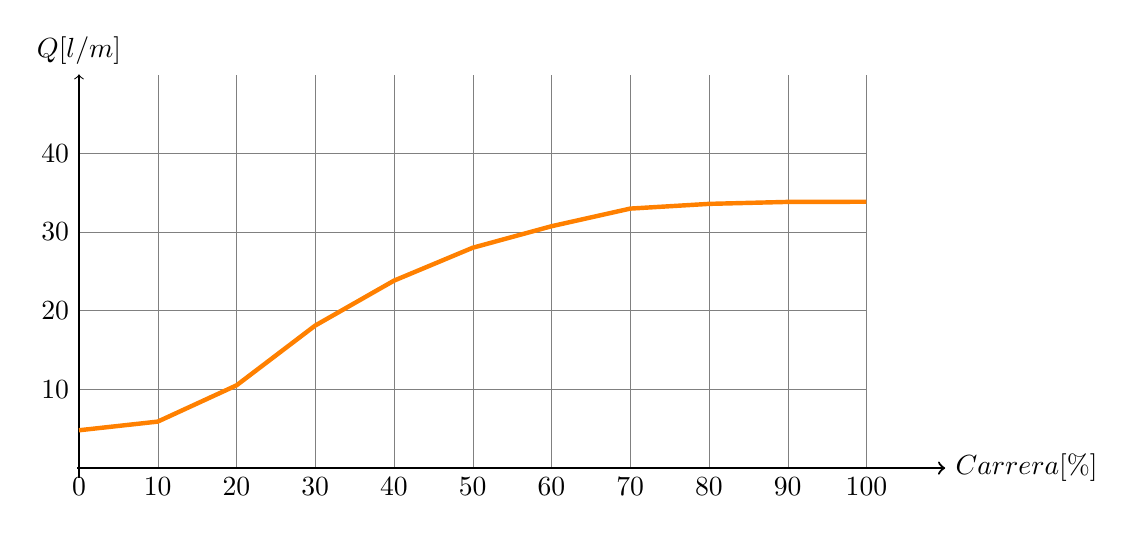
\begin{tikzpicture}[scale= 0.1, domain=0:110]
    
    \draw[ultra thin,color=gray,step=10cm] (100,49.9) grid (0.1,0.1);
    \draw[thick,->] (-0.2,0) -- (110,0) node[right,draw=none] {$Carrera [\%]$};
    \draw[->] (0,-1.2) -- (0,50) node[above,draw=none] {$Q [l/m]$};
    
    \foreach \x in {0,10,20,30,40,50,60,70,80,90,100}
    \draw (\x cm,1pt) -- (\x cm,-1pt) node[anchor=north,draw=none] {$\x$};
    \foreach \y in {10,20,30,40}
    \draw (1pt,\y cm) -- (-1pt,\y cm) node[anchor=east,draw=none] {$\y$};
    
    \draw[color = orange,ultra thick] (0,4.8) -- (10,5.9) -- (20,10.5)
    -- (30,18.1) -- (40,23.8) -- (50,27.98) -- (60,30.71)
    -- (70,32.95) -- (80,33.55) -- (90,33.8) -- (100,33.82);
   
\end{tikzpicture}
\caption{Característica efectiva de la válvula sin tiempo muerto.}
\label{fig:valvulaStiempoMuerto}
\end{figure}

\begin{figure}[ht]
  \centering
  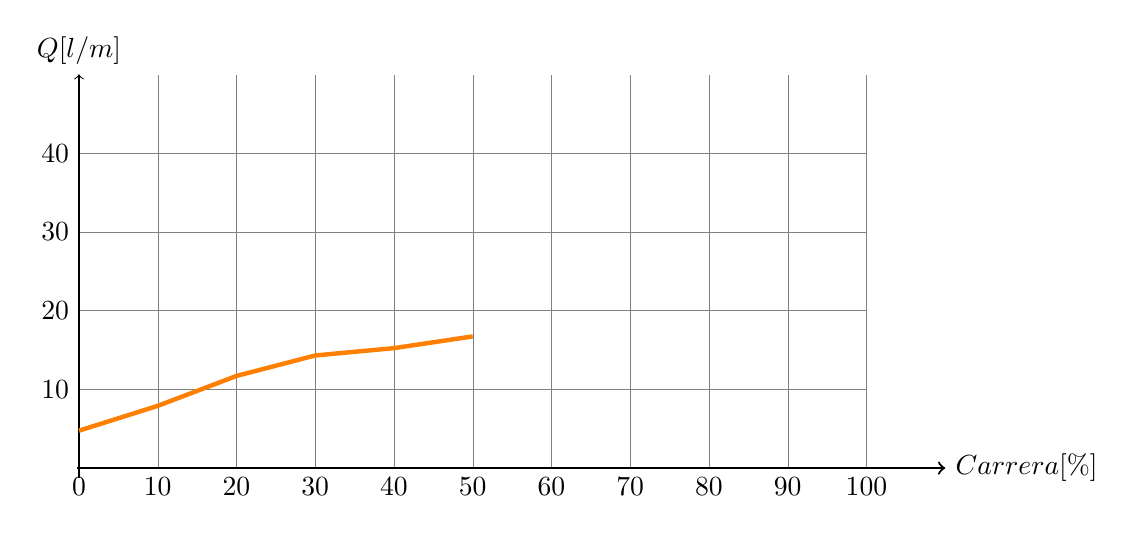
\begin{tikzpicture}[scale= 0.1, domain=0:110]
    
    \draw[ultra thin,color=gray,step=10cm] (100,49.9) grid (0.1,0.1);
    \draw[thick,->] (-0.2,0) -- (110,0) node[right,draw=none] {$Carrera [\%]$};
    \draw[->] (0,-1.2) -- (0,50) node[above,draw=none] {$Q [l/m]$};
    
    \foreach \x in {0,10,20,30,40,50,60,70,80,90,100}
    \draw (\x cm,1pt) -- (\x cm,-1pt) node[anchor=north,draw=none] {$\x$};
    \foreach \y in {10,20,30,40}
    \draw (1pt,\y cm) -- (-1pt,\y cm) node[anchor=east,draw=none] {$\y$};
    
    \draw[color = orange,ultra thick] (0,4.75) -- (10,7.9) -- (20,11.7)
    -- (30,14.3) -- (40,15.23) -- (50,16.72);
   
\end{tikzpicture}
\caption{Característica efectiva de la válvula con tiempo muerto.}
\label{fig:valvulaCtiempoMuerto}
\end{figure}

\subsection{Efecto de flujo estrangulado}

Luego de analizar los resultados obtenidos en la pruebas de la planta se pudo
constatar la presencia del efecto de flujo estrangulado o \emph{Choked
Flow}: se observa que la velocidad del fluido permanece constante, a partir de
una carrera del $70\%$.
Posteriores incrementos de la carrera no aumentan la velocidad del fluido en la
válvula.

Es una condición dinámica del fluido asociada con el efecto Venturi.
Cuando un flujo de fluido a una presión y temperatura dada pasa a través de una
restricción (por ejemplo: garganta, zona convergente/divergente o válvula),
la presión disminuye y la velocidad del fluido aumenta.
Considerando condiciones de fluidos subsónico, el principio de conservación de
masa exige que la velocidad del fluido aumente a medida que disminuye el diámetro 
de la garganta. Al mismo tiempo, el efecto Venturi ocasiona que la presión estática
y por lo tanto la densidad disminuyan luego de la restricción. El efecto de flujo
estrangulado es una condición limitante que se genera cuando el caudal no se 
incrementará con una disminución adicional en la presión aguas abajo de la 
restricción mientras la presión aguas arriba se mantiene constante.
\todo{Fuentes? No es por cavitación?}

\subsection{Montaje}
Dada la importancia y tamaño de la válvula, se colocó en el centro de
la planta, sobre la base de madera.
Al momento del montaje se tuvo especial atención en que se pudieran apreciar
con claridad las diferentes partes que la componen.
Se prestó especial atención al nivelado de la válvula.
Finalmente, se fijó mediante ménsulas a la base de madera y a la estructura
de caño.

\section{Instrumentos de Medición}
\label{sec:InstrumentosMedicion}
Para conocer el estado de la planta, es necesario tener conocimiento del
estado de varias variables de la planta, a saber:
\begin{itemize}
 \item \textbf{Nivel de los tanques}
 \item \textbf{Caudal en las tuberías}
 \item \textbf{Presión en las tuberías}
\end{itemize}
Debemos entonces, instalar elementos de instrumentación para poder 
medir y controlar estas variables de interés.

\subsection{DP Cell}
\label{subsec:DPCell}

Se denomina \textit{DP Cell}, o celda de presión diferencial, a un sensor
que mide la diferencia de presión entre dos puntos.\todo{Una foto chabon}
En nuestro caso, la celda entrega una corriente proporcional a la diferencia de
presión medida, en el rango de $4-20\,mA$.
Este valor de corriente será leído por el controlador de la planta.
Las DP cell utilizadas tienen las especificaciones que se muestran en la Tab.
\ref{tab:caractDPcell}.

\begin{table}
\centering
\begin{tabular}{|l|l|}
\hline
Marca & Yokogawa\\
Modelo & EJA 110 A\\
Sufijo & EMSOA - 22EN / FU1 / D4\\
Tensión & $10.5\,-\,30 \, DC$\\
Output & $4-20\,mA$\\
Presión máxima & $160\,bar$\\
Rango de calibración & $0$ a $10000\,mmCa$\\
\hline
\end{tabular}
\caption{Especificaciones de las celdas de presión diferencial.}
\label{tab:caractDPcell}
\end{table}

Dos celdas serán utilizadas:
\begin{itemize}
 \item \textbf{Medición del nivel del tanque:} una de las entradas de la celda
se conecta  al nivel más bajo del tanque y la otra a presión atmosférica.
La celda mide la presión debida al peso  de la columna de agua en el tanque.
Fue calibrada de manera que entregara un valor de corriente mínimo
cuando el tanque está vacío, y un valor máximo en el caso de que esté
lleno.
Así, el valor entregado por la celda es proporcional al nivel de
agua en el tanque.

\item \textbf{Medición del caudal en la tubería de llenado del tanque
controlado:}
Se utilizará una placa orificio para generar una caída de presión debida al
caudal.
Las entradas de la celda se conectan aguas arriba y aguas abajo
de la placa orificio.
Se mide de esta manera la diferencia de presión entre ambos puntos, que será
traducido en un valor de caudal en el
controlador (ver Sec. \ref{subsec:PlacaOrificio}).
\end{itemize}

Ambas celdas fueron fijadas a la base de madera mediante tornillos.
Las conexiones de las entradas se realizaron con mangueras de alta presión
malladas, de $6\,mm$.

Debemos destacar que, para el caso de la celda de caudal, ambas
entradas se conectaron entre si mediante una válvula manual.
Esta válvula se utiliza solamente durante el primer arranque de la planta:
cuando la cañería está vacía y la bomba B1 se activa, tenemos por una pequeña
fracción de tiempo una presión diferencial de $12\,mCa$ que puede dañar la
celda.
Para evitar este fenómeno, la válvula manual que conecta ambas entradas
permanece abierta durante el primer arranque.
Luego, debe cerrarse para poder realizar la lectura diferencial de presión.

\subsection{Placa Orificio}
\label{subsec:PlacaOrificio}
  se colocó en serie con la cañería de llenado del tanque controlado.
  Debieron instalarse además, las mangueras correspondientes de conexión 
  con la celda de presión diferencial.
  % El tablero se trata en el cap 3 :)
  %\item Tablero electrónico:
  %Estaba montado sobre la estructura una caja estanca donde se montaron todos 
  %los componentes eléctricos
  %y electrónicos.

Para medir el caudal en la tubería de ida, se decide
utilizar una placa orificio\todo{placa orif? u otra cosa?}.
En la Fig. \ref{fig:placaOrificio} se muestra un corte longitudinal de una placa
orificio.
Se observa que la placa orificio provoca una disminución del diámetro
de la cañería, con la consiguiente aceleración del fluido.
Escribiendo la ecuación de Bernoulli en 1 y 2\todo{verif. puntos}.

\begin{figure}
 \centering
 \missingfigure[figwidth=8cm]{Placa orificio}
 \caption{Corte longitudinal de una placa orificio montado en una tubería.}
 \label{fig:placaOrificio}
\end{figure}

\begin{align}
 z_1 \, \gamma + \dfrac{\rho \,v_1^2}{2} + P_1 &= z_2 \, \gamma + \dfrac{\rho \,v_2^2}{2} + P_2
\label{eq:Bernoulli}
\end{align}
donde $z_i$ y $P_i$ es la altura y presión en el punto $i$ y $\rho$ es 
la densidad del fluido. 
Considerando que la altura en ambos puntos es la misma, la ecuación
\eqref{eq:Bernoulli} puede reescribirse como
\begin{align}
 v_2^2 - v_1^2 &= 2\,g\,h_p
 \label{eq:Bernoulli2}
\end{align}
donde $h_p$ es la diferencia de presión entre 1 y 2, expresada como 
altura de la columna fluida
\begin{align}
 h_p &= \dfrac{P_1}{\gamma}-\dfrac{P_2}{\gamma}
\end{align}
La ecuación de continuidad, para fluidos incompresibles se escribe
\begin{align}
 A_1\,v_1 &= A_2\,v_2 \\
 v_2 &= \dfrac{A_1}{A_2} v_1 \\
 v_2 &= \dfrac{D_1^2}{D_2^2} v_1
 \label{eq:velRef}
\end{align}
y reemplazando \eqref{eq:velRef} en \eqref{eq:Bernoulli2} obtenemos
\begin{align}
 2 \, g \, h_p &= v_2^2 \left( 1 - \dfrac{D_1^4}{D_2^4} \right)\\
 \beta &= \dfrac{D_1}{D_2}\\
 v_2 &= \sqrt{\dfrac{2 \, g \, h_p}{1-\beta^4}}
\end{align}
finalmente, el caudal se obtiene multiplicando la velocidad $v_2$ por el
área $A_2$.
Además, se agrega un coeficiente $C_v$ debido al fenómeno de vena contracta:
\begin{align}
 Q &= \dfrac{C_v \, A_2}{\sqrt{1-\beta^4}}\, \sqrt{2 \, g \, h_p}
 \label{eq:placaOrif1}
\end{align}
El coeficiente $C_v$ depende del número de Reynolds $Re$ \cite{bib:Mataix, bib:ApuntesPuglesiPlacaOrif}
\begin{align}
Re &= \dfrac{D\,v}{\nu}
\end{align}
donde $v$ es la velocidad en la placa orificio, $D$ es el diámetro y ${\nu}$
es la viscosidad cinemática del fluido\footnote{Para el agua, nuestro fluido de
trabajo $\nu = 1,003\,10^{-6} \frac{m^2}{s}$.}

La ecuación \eqref{eq:placaOrif1} puede ser reescrita de una forma más sencilla
mediante una nueva variable adimensional $C_q$
\begin{align}
 C_q &= \dfrac{C_v}{\sqrt{1-\beta^4}}
\end{align}
$C_q$, por consiguiente depende tanto del número de Reynolds como de la razón
de los diámetros $\beta$. $C_q$ puede ser encontrado en tablas y ábacos en la
literatura \cite{bib:Mataix}.

No obstante, se observa que el valor de $C_q$ varia poco para valores de
$Re > 20000$, y depende fundamentalmente de $\beta$.
Por ende, puede ser considerado constante para una instalación dada.
Finalmente, la ecuación \eqref{eq:placaOrif1} puede ser expresada como
\begin{align}
 Q &= C_q\,A_2\, \sqrt{2\,g\,h_p}
\end{align}
que puede ser reescrita, teniendo a $C_q$ constante
\begin{align}
 Q &= K\,\sqrt{h_p}
 \label{eq:placaOrifPLC}
\end{align}
donde se observa que el caudal $Q$ es proporcional a la raíz cuadrada de
la diferencia de alturas $\sqrt{h_p}$, que puede
ser encontrada utilizando un DP cell (ver Sec. \ref{subsec:DPCell}).

\subsubsection{Metodología experimental}
Considerando $C_q$ constante,
\begin{align}
 K = C_q\, A_2\, \sqrt{2\,g}
\end{align}
es constante también, y puede ser determinado experimentalmente.
Para ello, se midió sobre el tanque controlado una distancia $l$.
Luego, se encendió la bomba B1 con la válvula electroneumática en posición
abierta (caudal máximo), y se midió el tiempo $t$ necesario para que el nivel
alcanzara la altura $l$.
Ya que el tanque tiene un diámetro $D$, el caudal máximo puede ser
calculado como
\begin{align}
 Q_{max} &= \dfrac{\pi\,D^2\,l}{4\,t}
\end{align}

El módulo analógico del \gls{plc} tiene una resolución de $12\,bits$
(ver Sec. \ref{subsec:plc}), un valor de caudal máximo corresponde a $h_f =
4095$.
$K$ se calcula como
\begin{align}
 K &= \dfrac{Q_{max}}{\sqrt{4095}}
\end{align}
Luego, el caudal puede calcularse fácilmente aplicando la ecuación
\eqref{eq:placaOrifPLC}.

Para la determinación del valor de $K$ se trabajó sin tiempo muerto.
Se marcó en el tanque controlado una altura $l=0.5\,m$, teniendo $D=0.2\,m$.
Luego, se procedió a medir el tiempo de llenado, consignando los resultados en
la Tab. \ref{tab:tiempoK}.

\begin{table}
  \centering
  \bgroup
%   \scriptsize
%   \def\tabcolsep{6.50pt}
%   \def\arraystretch{1.22}%
  \begin{tabular}{|c|c|}
  \hline
  Medición & Valor\\
  \hline
  1 & $27.27\,s$ \\
  2 & $28.53\,s$ \\
  3 & $27.98\,s$ \\
  4 & $28.10\,s$ \\
  5 & $27.68\,s$ \\
  6 & $27.66\,s$ \\
  \hline
  \hline
  \textbf{Media} & $27,87\,s$\\
  \textbf{SD} & $0.43\,s$\\
  \hline
  \end{tabular}
  \egroup
  \caption{Medición del tiempo de llenado, cálculo de $K$.}
  \label{tab:tiempoK}
\end{table}

Finalmente, obtenemos
\begin{align}
 Q_{max} &= 33.81\,\dfrac{lts}{min}
 \\
 K  &= 0.5285\,\dfrac{lts}{min}
\end{align}

\subsection{Manómetros}
\label{subsec:Manometros}

\begin{figure}[ht]
 \centering
 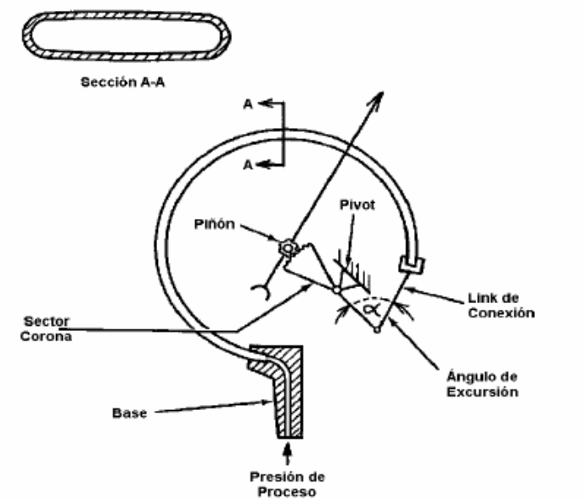
\includegraphics[width=.7\textwidth]{Cap2-DisenoEnsamblado/images/manomBourdon.png}
 \caption{Manómetro de Bourdon, extraído de \cite{bib:ApuntesPuglesiPlacaOrif}}
 \label{fig:manometroBourdon}
\end{figure}

Para conocer los valores de presión en ambas cañerías
(referirse al \gls{pyid}, Sec. \ref{sec:p&id}),
se instalaron manómetros comunes, de tipo Bourdon.
Un ejemplo de estos manómetros se muestra en la Fig. \ref{fig:manometroBourdon}.
Se observa que un incremento de la presión produce una deformación
del \emph{tubo de Bourdon}, reflejado en la aguja indicadora.
El manómetro de Bourdon permite obtener una medición visual de la
presión relativa, del punto donde se encuentra instalado.

Durante el montaje, se presentó el problema que uno de los manómetros
no entregaba una medición definida, sino que oscilaba alrededor de un
valor medio (imposibilitando la lectura directa).
Este problema fue solucionado instalando un \textbf{manómetro con glicerina},
donde el mecanismo del manómetro se encuentra sumergido en un baño de glicerina.
Debido a la viscosidad del fluido, las vibraciones quedan amortiguadas
y el manómetro refleja el valor medio de la presión.

Las especificaciones de los manómetros se muestran en la Tab,
\ref{tab:EspManoms}.

\begin{table}[ht]
\centering
\begin{tabular}{|l|l|}
\hline
Marca & Beyca\\
Rango & $0$ - $1\,kgf/cm^2$\\
 & $0$ - $14\,lb/pulg^2$\\
Escala & $0.02\,kgf/cm^2/div$\\
& $0.5\,lb/pulg^2/div$\\
\hline
\end{tabular}
\caption{Especificaciones de los manómetros}
\label{tab:EspManoms}
\end{table}

\chapter{Tablero Eléctrico y Conexionado}
\label{ch:tablero}

Luego del diseño y ensamblado de los componentes de la planta, descripto en el
Cap.
\ref{ch:DisenoEnsamblado}, se procedió al diseño y montaje del
tablero eléctrico.
Es decir, se realizó la instalación y el cableado de los elementos eléctricos y
electrónicos.
Para comprender este capítulo es imprescindible utilizar los diagramas
del tablero, que pueden encontrarse en el anexo \ref{anexo:diag}.
Por simplicidad, se dividirá el análisis del tablero en dos secciones:
\begin{itemize}
 \item \textbf{Potencia:} corresponde a la instalación y el cableado
 de los elementos eléctricos de la planta, destinados a alimentar los motores de
 las electrobombas y los circuitos lógicos.
 \item \textbf{Señal:} corresponde a la instalación y el cableado
 de los elementos electrónicos cuyo objetivo es controlar la planta.
 Podemos citar: \gls{plc}, módulos inalámbricos,
 transmisores de presión y caudal, actuadores (válvula de control).
\end{itemize}

\section{Potencia}
\label{sec:Potencia}
Tal como se describió previamente, los elementos de potencia deben
\textbf{alimentar} los motores y elementos lógicos de la planta.
Se optó por trabajar con corriente alterna monofásica ($220\,V\,-\,50\,Hz$),
dado que es la alimentación de las electrobombas.
En el anexo \ref{anexo:diag}, se muestran los conductores de fase y neutro en
colores marrón y azul respectivamente.
Los elementos de potencia se describen a continuación.

\subsection{Corte General}
\label{subsec:corteGeneral}
El primer elemento que encontramos en el tablero es el interruptor
termomagnético de corte general (ver folio 1 del diagrama de tablero).
El interruptor es bipolar (neutro y fase), modelo \verb|C60 N|, número de
referencia \verb|24335| y marca Merlin Gerin (Schneider).
Se trata de un termomagnético para cargas convencionales, con una corriente
nominal $I_n$ de $6\,A$ y una corriente de corte por cortocircuito de $5$ a
$10\,I_n$.

La función del termomagnético es proteger la instalación frente a posibles
sobrecargas (mediante la interrupción del circuito térmico) y cortocircuitos
(mediante la interrupción del circuito magnético).
Además, es utilizado como llave de corte general para encender o apagar la
planta.

\subsection{Alimentación de los Motores de las Electrobombas}
\label{subsec:alimentacionMotores}
Puede verse el esquema de alimentación de los motores en los folios 1 y 2 del
anexo \ref{anexo:diag}.
Para cada una de las electrobombas, se utilizaron los siguientes elementos de
protección y comando:
\begin{itemize}
 \item \textbf{Relés:}
 los relés reciben una señal de activación de $24\,V$, de parte del PLC.
 Al activarse, el relé entrega en el borne \verb|11 (7)| una señal de $220\,V$
de corriente alterna.
Esta señal alimentará la bobina de los los contactores de los motores, previo 
paso por el relevo térmico. Se utilizaron relés \verb|LZX:PT 370| de Siemens.
 \item \textbf{Relevo Térmico:}
 tiene como objetivo evitar la sobrecorriente en los motores.
 Para el proyecto, se configuró el relevo térmico con una corriente
 de $1.6\,A$.
 En caso de superar este valor, interrumpe tensión en la bobina
 del contactor y se detienen los motores.
 Se utilizaron relevos térmicos \verb|LRD 06| de Telemecanique, conectados
inmediatamente después del relé.
 \item \textbf{Contactores:}
 encienden los motores, a partir de una señal de activación de $220\,V$ de
corriente alterna.
Se utilizaron contactores \verb|LC1-D09| de Schneider Electric.
Debido a que los contactores son trifásicos, debió realizarse un bucle con dos
de las fases (ver diagrama del tablero).
\end{itemize}

En la Fig. \ref{fig:diagramaLadderContactor} se muestra el diagrama ladder
del conexionado de los motores.
Se observa que  el motor estará encendido si la bobina del relé esta activada y
si el relevo térmico no acusa sobrecorriente.

\begin{figure}
 \centering
 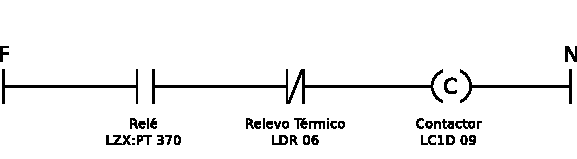
\includegraphics[scale=1.1]{Cap3-TableroElectrico/Images/ladderConexion.pdf}
 \caption{Esquema Ladder del conexionado de los motores.}
 \label{fig:diagramaLadderContactor}
\end{figure}

\subsection{Fuente de alimentación}
\label{subsec:fuenteAlim}
Los circuitos lógicos de la planta (\gls{plc}, transmisores de señal) funcionan con una
tensión de $24\,V$ de corriente continua.
Se optó por utilizar una fuente de alimentación industrial para energizar estos
circuitos lógicos.
Las características técnicas de la fuente se muestran en la Tab.
\ref{tab:fuenteAlim}.
\begin{table}[h]
\renewcommand{\arraystretch}{1.3}
\centering
\begin{tabular}{|l|l|}
\hline
Marca & ReignPower\\
Tensión Entrada& $100-120$ / $200-240\,V$\\
Tensión Salida& $24\,V$\\
Corriente Salida Máxima& $4.2\,A$\\
Potencia & $100\,W$\\
\hline
\end{tabular}
\caption{Características de la fuente de alimentación.}
\label{tab:fuenteAlim}
\end{table}

En el diagrama de tablero, se muestran los conductores de $+24\,V$ y $0\,V$ en
rojo y negro respectivamente.
La fuente de alimentación se muestra en el folio 1.

\section{Señal}
\label{sec:Senal}

El circuito de señal tiene como objetivos:
\begin{itemize}
 \item Captar variables de la planta (caudal, presión), procesarlas y entregar
consignas a la válvula de control.
\item Activar los relés descriptos en la Sec.
\ref{subsec:alimentacionMotores} para encender o apagar los motores de las
electrobombas.
\item Conectar la planta a una computadora supervisora (\gls{scada}), para poder
supervisar su estado como así también recibir señales de control.
\end{itemize}

\subsection{PLC}
\label{subsec:plc}

\glsreset{plc}
Para automatizar la planta se optó por utilizar un \gls{plc} Twido
\verb|TWD LMDA 40 DTK| de Schneider.
Se trata de un sistema electrónico digital de automatización y control, pensado
para aplicaciones industriales, seguro frente a condiciones adversas,
vibraciones e interferencias radioeléctricas \cite{bib:ApuntesJGabriel}.
El autómata se adapta al proceso a controlar mediante un
\textit{software} o programa de aplicación específico, que contiene la secuencia
de operaciones a realizar.
Se pueden utilizar las entradas, los valores en memoria y valores
recibidos mediante un bus de comunicaciones del autómata para modificar el
estado de las salidas \cite{bib:libroAutomat1}.

Un \gls{plc} está conformado por los siguientes elementos:
\begin{itemize}
 \item \textbf{Procesador:} en función de los valores de los sensores discretos
y transmisores continuos (entradas) y de la información almacenada,
genera señales hacia los
actuadores
(salidas).
El procesador sigue un algoritmo, denominado programa de aplicación,
que indica la secuencia de operaciones a realizar.
Entre los lenguajes de programación definidos en la norma \verb|IEC 61131|
podemos citar: Ladder, Texto Estructurado, Lista de Instrucciones y GRAFCET
(SFC).
 \item \textbf{I/O discretas:} las entradas y salidas discretas se
utilizan para acciones de control discretas, tal como encender motores
o leer sensores discretos (fines de carrera, pulsadores, señales binarias).
En este proyecto, se utilizan las salidas discretas \verb|Q0.0| y \verb|Q0.1|
para activar los relés de los motores.
Además \verb|I0.0| e \verb|I0.1| se
utilizan como señales de enclavamiento: conectadas a los contactores, verifican
que el motor se encuentre efectivamente encendido.
Se pueden observar estas señales de control en los folios 1 y 2 del diagrama de
tablero.
Además, se muestra el esquema de conexionado del \gls{plc} en el folio
3 del diagrama de tablero.
\item \textbf{I/O analógicas:} mediante una entrada
analógica, se pueden leer
señales de corriente ($4-20\,mA$) o tensión ($0-10\,V$) provenientes de los
transmisores de señal.
De la misma manera, las salidas analógicas permiten enviar consignas
de tensión o corriente a los actuadores.
En este proyecto, las entradas analógicas \verb|IW0.1.0| e \verb|IW0.1.1|
permiten leer los valores de los DP cell de nivel y caudal, respectivamente.
Se emplea la salida analógica \verb|QW0.1.0| para controlar el
electroposicionador.
Cabe destacar que el \gls{plc} no posee I/O analógicas.
Por ello, debió anexarse un módulo \verb|TWD AMM 6HT|.
La resolución de lectura máxima de las entradas analógicas es de $12\,bits$,
con un tiempo de muestreo de $16\,ms$.
Se pueden ver estas señales de control en el folio 4 del diagrama de tablero.

\item \textbf{Comunicación:} El puerto de comunicaciones permite programar el 
controlador, como así también enviar comandos y recibir información de
la planta durante la ejecución con el \gls{scada}.
El \gls{plc} utilizado cuenta con un puerto de comunicaciones \verb|RS-485|.
Se presentan dos opciones para la conexión con la computadora supervisora:
\begin{itemize}
 \item Mediante una conexión cableada:
 se conecta el puerto \verb|RS-485| a un puerto \verb|RS-232C| de la computadora
mediante un adaptador específico, fabricado durante el desarrollo del
proyecto\footnote{En este caso, dado que la computadora no contaba con un
puerto serie, se utilizó un adaptador
\texttt{USB} a \texttt{RS-232C}.}.
Se muestra en el anexo \ref{anexo:circuitos}, folio 1, el circuito esquemático
utilizado.
Además, se incluyen los diseños de PCB para replicar el circuito.

No obstante, utilizar una conexión cableada impone un vínculo físico entre
el \gls{plc} y la computadora supervisora (impidiendo que la planta sea móvil).
\item Mediante un módulo de comunicación inalámbrica:
descripto en la Sec. \ref{subsec:inalambrico}.
\end{itemize}
\end{itemize}

\subsection{Módulos inalámbricos}
\label{subsec:inalambrico}

Para comunicar la planta con la computadora supervisora, sin necesidad de
utilizar un cable de par trenzado, se decidió utilizar un módulo inalámbrico
\verb|ADC-200| de CTM Electrónica (ver Fig. \ref{fig:fotoModuloIn}).
Se trata de un equipo de comunicaciones para realizar enlaces inalámbricos que
utilicen la interfaz \verb|RS-232C| o \verb|RS-485|.
Se muestran las características técnicas relevantes en la Tab.
\ref{tab:caractMod}.

\begin{figure}[t]
\centering
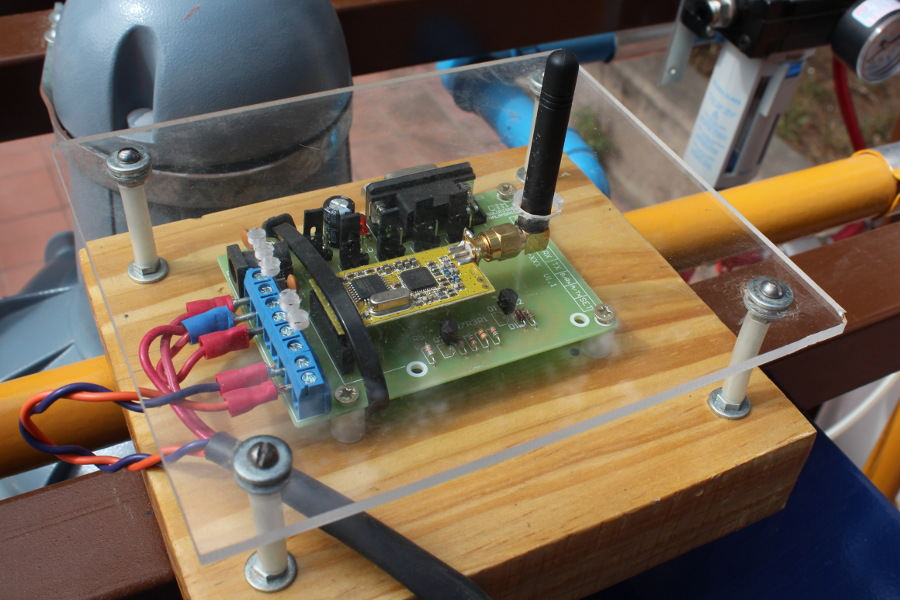
\includegraphics[width=.6\textwidth]{Cap3-TableroElectrico/Images/IMG_5038.JPG}
 \caption{Módulo inalámbrico montado sobre la estructura.}
 \label{fig:fotoModuloIn}
\end{figure}

\begin{table}[ht]
\renewcommand{\arraystretch}{1.3}
\centering
\begin{tabular}{|l|l|}
\hline
Alimentación & $5\,VCC$\\
Consumo& $60\,mA$\\
Alcance& $1000\,m$\\
Baud Rate &2400 a 19200 bps \\
Frecuencia& 431 a 470 Mhz en más de 100 canales\\
\hline
\end{tabular}
\caption{Características de los módulos inalámbricos.}
\label{tab:caractMod}
\end{table}

Para el proyecto, se conectó el módulo tal como lo indica el
diagrama de tablero (folio 5), estipulando una velocidad de transferencia de
\verb|19200 bps|, sin pariedad, con un bit de stop.

Además, dado que el módulo inalámbrico debe alimentarse con una tensión de
$5\,V$ de corriente continua, se desarrolló una fuente conversora de $24\,V$ a
$5\,V$ basada en el integrado \verb|LM7805|.
El circuito esquemático de la fuente puede encontrarse en el folio 2 del anexo
\ref{anexo:circuitos}.
Además, se incluye el diseño del PCB para poder replicar el circuito.

Cabe destacar que el módulo inalámbrico \textbf{no puede utilizarse} para
la programación del \gls{plc}, debido a que el software (Twido Soft) acusa un
error de timeout.
No obstante, su funcionamiento es correcto para recibir información
del estado de la planta y enviar consignas mediante el \gls{scada}.

\section{Imagen del tablero}

\begin{figure}[t]
        \centering
        \begin{subfigure}[b]{0.48\textwidth}
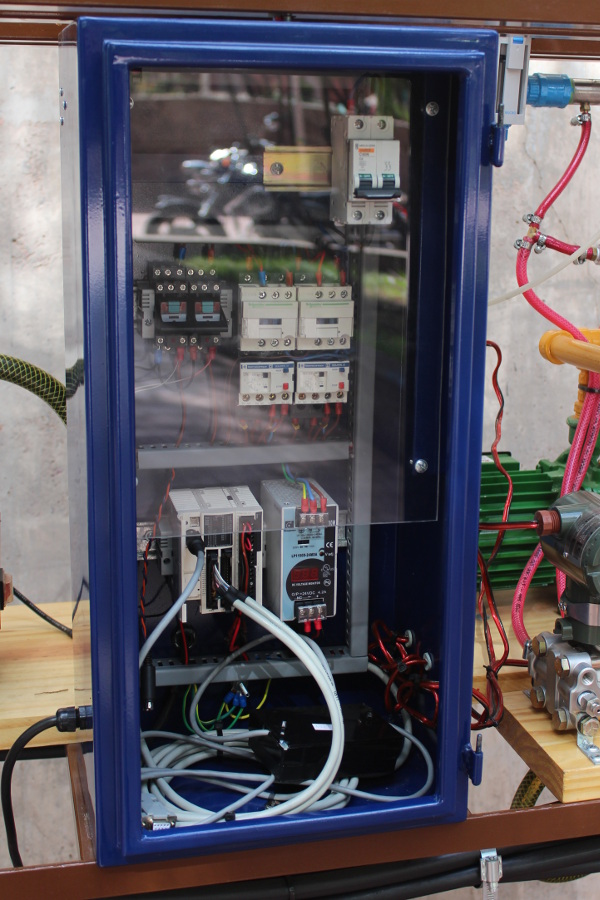
\includegraphics[width=\textwidth]{Cap3-TableroElectrico/Images/IMG_5074.JPG}
 \caption{Con acrílico de protección.}
 \label{fig:fotoTableroAcr}
        \end{subfigure}%
\hfill
\begin{subfigure}[b]{0.48\textwidth}
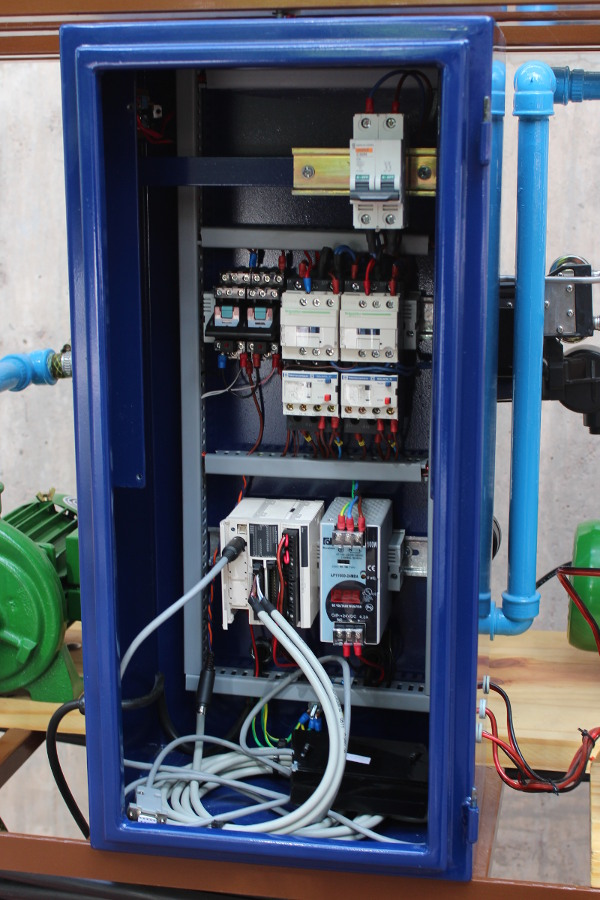
\includegraphics[width=\textwidth]{Cap3-TableroElectrico/Images/IMG_5097.JPG}
 \caption{Sin acrílico de protección.}
 \label{fig:fotoTableroSAcr}
        \end{subfigure}
        \caption{Fotografía del tablero finalizado.}
        \label{fig:fotoTablero}
\end{figure}

En la Fig. \ref{fig:fotoTablero} se muestran fotografías del tablero finalizado.
Pueden observarse tres niveles diferenciados:
\begin{itemize}
 \item En el nivel superior se encuentra el interruptor termomagnético de corte
general descripto en la Sec. \ref{subsec:alimentacionMotores}.
Este interruptor debe ser accionado para encender la planta.
\item En el nivel medio se encuentran los relés, contactores y relevos térmicos
para accionar los motores de las electrobombas (Sec.
\ref{subsec:alimentacionMotores}).
\item En el nivel inferior está el
\gls{plc}, con su módulo de E/S analógicas (Sec. \ref{subsec:plc}), y la fuente
de alimentación de $24\,V$ (Sec.
\ref{subsec:fuenteAlim}).
\end{itemize}
Los elementos fueron montados sobre
rieles DIN.  Todos los elementos, a excepción del interruptor
termomagnético, se encuentran protegidos por un acrílico transparente para
evitar accidentes (ver Fig. \ref{fig:fotoTableroAcr}).

\chapter{Programación PLC}
\label{ch:progPLC}

\section{Algoritmo}
\label{sec:Algoritmo}

\section{Programación}
\label{sec:Programacion}
Grabado y puesta en el plc

\begin{table}[!t]

\renewcommand{\arraystretch}{1.3}
\centering
\begin{tabular}{c||c}
\hline
\bfseries Memoria & \bfseries Descripción\\
\hline \hline
\verb|M0|  & Bandera de inicialización\\
\verb|M1|  & Lectura DP cell caudal\\
\verb|M2|  & Valor Kp\\
\verb|M3|  & Valor Ki\\
\verb|M4|  & Valor Kd\\
\hline
\end{tabular}
\caption{Banderas internas}
\end{table}

\begin{table}[!t]

\renewcommand{\arraystretch}{1.3}
\centering
\begin{tabular}{c||c||c||c}
\hline
\bfseries Tipo & \bfseries Word & \bfseries Bit & \bfseries Descripción\\
\hline \hline
Lect & \verb|MW0| & \verb|X0| & Señal Run PLC\\
Lect & & \verb|X1| & Alarma HHL\\
Lect & & \verb|X2|& Alarma LLL\\
Lect & & \verb|X3|& Alarma HL\\
Lect & & \verb|X4|& Alarma LL\\
Lect & & \verb|X5|& Error en motores (era \verb|MW0:X13|)\\
Lect & & \verb|X6|& Motor 1 encendido (era \verb|MW0:X11|)\\
Lect & & \verb|X7|& Motor 2 encendido(era \verb|MW0:X12|)\\
Lect & & \verb|X8|& Modo manual activado (era \verb|MW0:X14|)\\
Lect & & \verb|X9|& Modo automático activado y funcionando (Nuevo)\\
Lect & & \verb|X10|& Planta funcionando sin errores (era \verb|MW0:X15|)\\
\hline
Esc & \verb|MW1| & \verb|X0|& Switch modo manual/automático (era 
\verb|MW0:X10|)\\
Esc & & \verb|X1|& Aplicar (era \verb|MW0:X15|)\\
Esc & & \verb|X2|& Encender/Apagar (automático) (era \verb|MW0:X9|)\\
Esc & & \verb|X3|& Se desea cambiar el PID (era \verb|MW0:X6|)\\
Esc & & \verb|X4|& Se desean los valores por default para el PID (era 
\verb|MW0:X7|)\\
Esc & & \verb|X5|& Se desean valores por default para SP (era \verb|MW0:X8|)\\
Esc & & \verb|X6|& Encender M1 (manual) (era \verb|MW8:X1|)\\
Esc & & \verb|X7|& Encender M2 (manual) (era \verb|MW8:X2|)\\
Esc & & \verb|X8|& Limpiar errores (era \verb|MW8:X0|)\\
\hline

\hline
\end{tabular}
\caption{Bits lectura/escritura}
\end{table}

\begin{table}[!t]

\renewcommand{\arraystretch}{1.3}
\centering
\begin{tabular}{c||c||c}
\hline
\bfseries Tipo & \bfseries Word  & \bfseries Descripción\\
\hline \hline
Lect & \verb|MW2|  & Lectura DP cell nive (era \verb|MW1|)\\
Lect & \verb|MW3|  & Lectura DP cell caudal\\
Lect & \verb|MW4|  & Valor Kp\\
Lect & \verb|MW5|  & Valor Ki\\
Lect & \verb|MW6|  & Valor Kd\\
Lect & \verb|MW7|  & Valor de lectura del SP (era \verb|MW2|)\\
Lect & \verb|MW8|  & Valor de lectura de la válvula (era \verb|MW7|)\\
\hline
Esc & \verb|MW9| & Valor de escritura de la válvula (manual) (era 
\verb|MW15|) \\
Esc & \verb|MW10|  & Valor de escritura del SP \\
Esc & \verb|MW11|  & Valor de escritura Kp \\
Esc & \verb|MW12|  & Valor de escritura ki) \\
Esc & \verb|MW13| & Valor de escritura Kd \\
\hline
\end{tabular}
\caption{Palabras lectura/escritura}
\end{table}

\section{Depuración (Debug)}
\label{sec:Debug}
Forzar entradas

\chapter{SCADA}
\label{ch:scada}

%Finalmente y para resumir la evolución del proyecto hasta este punto
Para continuar en el desarrollo es necesario analizar los pasos antes descriptos para la construcción
de la planta. De esta manera, en el capitulo \ref{ch:DisenoEnsamblado} detallamos el sistema 
físico, lo que nos conduce a describir en el capitulo \ref{ch:tablero} el sistema eléctrico y
electrónico que anima a la planta, continuando en el capitulo \ref{ch:progPLC} con la lógica
que regula al sistema completo por medio del \gls{plc}. 

Como elemento final del \gls{pfe} se diseño y realizo una \gls{hmi} \gls{scada}
mediante P-CIM para Windows de AFCON con el objetivo de poder manipular la planta/el sistema
sin tener un acceso físico a la misma.

En el siguiente capítulo se detallan cada uno de los pasos seguidos para la realización de tal 
interfaz así como también la configuración actual. Mediante esta información el lector podrá entender
y por lo tanto modificar en caso de ser necesario el entorno. Sin embargo, este capitulo no esta 
orientado a la operación misma de la planta mediante el \gls{scada} lo cual se detalla en la sección
\todo{agregar la sección donde se describe la operación mediante el scada}

\section{Introducción a SCADA}
\label{sec:IntroScada}

Aunque un \gls{plc} realiza automáticamente un control pre-programado sobre un proceso, 
no tienen una manera estándar de presentar la información al operador y ademas estos se 
distribuyen a lo largo de toda la planta, haciendo difícil recoger los datos de manera 
manual.%para poder concentrarlos
En cambio, los sistemas \gls{scada} obtienen los datos desde el \gls{plc} o desde otros controladores 
por medio de algún tipo de red y de manera automática, facilitando la tarea de concentrar los datos.
Se puede observar en la Fig.\ref{fig:perspectivaSCADA} de manera esquematica la organizacion 
de un sistema Planta-PLC-SCADA.
\begin{figure}[ht!]
	\centering
	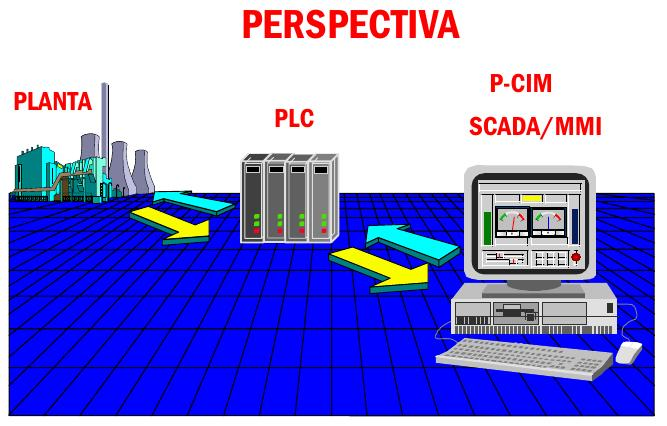
\includegraphics[width=0.445\textwidth]
	{Cap5-SCADA/images/perspectiva.jpeg}
	\caption{Diagrama de un sistema SCADA}
	\label{fig:perspectivaSCADA}
\end{figure}

Un sistema \gls{scada} recopila constantemente información de la planta en tiempo real. Luego en 
la base de datos se almacenan y evalúan los datos, también se generan alarmas en los casos 
correspondientes. Finalmente, mediante la \gls{hmi} se brinda la información al operario y 
este a su vez puede enviar instrucciones a los \gls{plc} en la planta. 
También se pueden incluir datos de diagnóstico y manejo de la información así como un cronograma 
de procedimientos de mantenimiento, información logística, esquemas detallados para un sensor 
o máquina en particular o incluso sistemas expertos con guía de resolución de problemas. Es 
entonces claro que la utilización de un sistema \gls{scada} reduce fuertemente las tareas asociadas al control
y monitoreo de plantas industriales.
 

\section{Scada P-CIM}
\label{sec:ScadaPCIM} 
Para el diseño y desarrollo del sistema \gls{scada} de este \gls{pfe} se utilizó el software 
P-CIM 7.70 SP4 para Windows de AFCON (\url{www.afcon-inc.com}). El mismo, provee de un ambiente 
tanto de desarrollo como de ejecución de aplicaciones \gls{scada}. Este software puede ser 
descargado desde la pagina de 
\href{http://www.afcon-inc.com/Templates/showpage.asp?TMID=108&FID=733&PID=0&IID=8334}{P-CIM 7.70 SP4}.

Dentro de las características del sofware P-CIM se encuentran:
\begin{itemize}
 \item Compatible con todas las plataformas MS-Windows actuales.
 \item Soporta un gran número de diferentes \gls{plc} y otros dispositivos periféricos.
 \item Posee drivers para diversos buses de comunicación.
 \item Provee herramientas para el desarrollo de \gls{hmi} inteligentes 
 \item Permite el seguimiento de los procesos de la planta y las actividades de los operadores
 \item Brinda un entorno para monitorear alarmas y eventos en toda la extensión de la planta
\end{itemize}


\subsection{Estructura de P-CIM}
\label{sec:CapasPrograma}
Como se puede observar en la Fig.\ref{fig:estructuraSCADA} la estructura de P-CIM se divide en tres 
grandes capas de abstracción:
\begin{figure}[ht!]
	\centering
	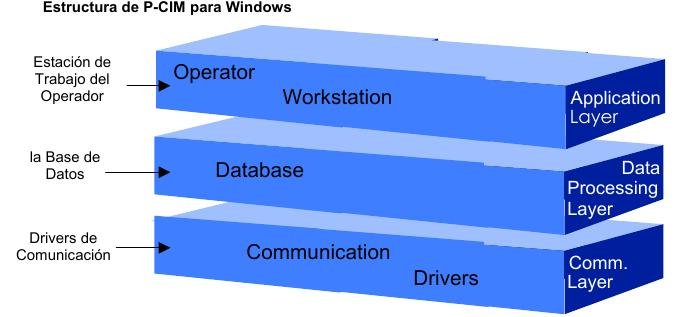
\includegraphics[width=0.445\textwidth]
	{Cap5-SCADA/images/estructura.jpeg}
	\caption{Esquema de la estructura en capas de P-CIM}
	\label{fig:estructuraSCADA}
\end{figure}

\begin{itemize}
 \item Capa de Comunicación: Se encarga de la comunicación entre el \gls{plc} y la PC.
 \item Capa de Procesamiento de Datos: Donde se lleva a cabo la mayor parte del procesamiento 
 de datos, registro histórico y manejo de alarmas.
 \item Capa de aplicación: Presenta la información, interactúa con el operador y realiza 
 los controles de alto nivel y de programación.
\end{itemize}

El trabajo coordinado se resume en que la información de campo del PLC llega al \gls{scada} a 
través de la capa de comunicación. Esta se transfiere a la Capa de Procesamiento de Datos (Servidor 
de la Base de Datos o Database Server) donde se analiza. La capa de aplicación la procesa y envía 
hacia la \gls{hmi}. De esta manera el funcionamiento conjunto de cada una de estas capas permite 
al sistema \gls{scada} funcionar de manera correcta y con las prestaciones antes mencionadas.


\section{Desarrollo de la aplicacion SCADA con P-CIM}
A continuación, se detalla la aplicación \gls{scada} desarrollada para este \gls{pfe} en el 
software P-CIM. Su exposición esta dividida de acuerdo a la estructura en capas del programa,como 
se describió en la sección \ref{sec:CapasPrograma}.

\subsection{Capa de comunicación}
\label{subsec:CapaComunicacion}
El primer paso para el desarrollo de un sistema \gls{scada} es lograr la comunicación por medio
de algún bus con el \gls{plc} que controla la planta. Es decir, lograr un buen funcionamiento de 
la capa de comunicación. 
En nuestro caso se utilizó el protocolo de comunicaciones Modbus. 

\subsubsection{Modbus}
Modbus es un protocolo de comunicaciones diseñado en 1979 por Modicon para su gama de \gls{plc}.
En abril del 2004, Schneider Electric transfirió los derechos a la la Modbus Organization 
\url{http://www.modbus.org/}, la cual se encarga desde entonces del desarrollo y actualización 
del protocolo Modbus.

Para la conexión entre un computador corriendo un software \gls{scada} y uno o varios \gls{plc} 
el protocolo Modbus es un estándar de facto en la industria . Por esta razón, también, 
goza de una gran disponibilidad para la conexión de dispositivos electrónicos industriales. 
A nivel diseño, se encuentra situado en la capa de aplicación según el modelo \gls{osi} y 
presenta una arquitectura maestro/esclavo o cliente/servidor.

Las principales razones para el uso de Modbus:
\begin{itemize}
 \item Simple y robusto
 \item Fue desarrollado para aplicaciones industriales.
 \item Su implementación es fácil y requiere poco mantenimiento.
 \item Maneja bloques de datos sin suponer restricciones a los vendedores.
 \item Permite la comunicación entre múltiples dispositivos en la misma red. Aprox. 240
 \item De código abierto y libre de regalías.%openly published and royalty-free
\end{itemize}


\subsubsection{Instalación Driver Modbus}
A continuación se detalla el  proceso de configuración y puesta en marcha del bus de comunicaciones. 
El driver de para Modbus se puede descargar desde esta 
\href{http://www.afcon-inc.com/afcon/Templates/showpage.asp?TMID=402&FID=832}{pagina}.
Para realizar la instalación de este driver de comunicaciones en P-CIM seguimos los siguientes pasos: 

% \begin{enumerate}
%  \item Elija $Setup~de~P-CIM$ del grupo de aplicaciones que se encuentran la carpeta $AFCON~P-CIM[7.70SP4]$.
%  \item Aparecerá en la pantalla la ventana de $Setup~de~P-CIM$. Elija $Install~P-CIM~Driver$.
%  \item La ventana de diálogo de instalación del Driver de P-CIM, le pedirá que indique el directorio del driver.
%        Oprima Browse.
%  \item Seleccione el directorio de origen del driver para Modbus. En nuestro caso $C:/P-CIM32.BAK/DRIVERS/MODBUS.689$.
%  Oprima OK y luego Next.
%  \item El Setup de P-CIM despliega la ventana de diálogo de Bienvenida. Para continuar, oprima Next. 
%  \item El Setup de P-CIM despliega la ventana de diálogo de Propiedades del Driver de P-CIM 
%   para Windows 32, indicando los detalles del driver a ser instalado.
%  \item Elija el/los proyecto(s) en los que Ud. desea instalar el driver o bien seleccione
%   All (todos) y oprima Next.
%   \item El Setup de P-CIM procede a efectuar la instalación y finalmente muestra este mensaje: 
%   “La instalación del driver se ha completado”. Oprima OK para que desaparezca el cuadro de diálogo.
% \end{enumerate}

\begin{table}[H]
\small
\centering
\renewcommand*{\arraystretch}{0.3}
\begin{tabular}{*{2}{m{0.45\textwidth}}}
\hline
  Elija Setup de P-CIM del grupo de aplicaciones que se encuentran la carpeta 
  AFCON P-CIM[7.70SP4]. Luego seleccione Install P-CIM Driver.
  &\begin{center}
    \rule{0.4\textwidth}{0.3\textwidth}
  \end{center}\\
\hline
  La ventana de diálogo de instalación del Driver de P-CIM, le pedirá que 
  indique el directorio del driver.
       Oprima Browse.
  &\begin{center}
    \rule{0.4\textwidth}{0.3\textwidth}
  \end{center}\\
\hline
  Seleccione el directorio de origen del driver para Modbus. En nuestro caso 
  \texttt{C:\slash P-CIM32.BAK\slash DRIVERS\slash MODBUS.689}. Oprima OK y 
luego Next.
  &\begin{center}
    \rule{0.4\textwidth}{0.3\textwidth}
  \end{center}\\
\hline
 Se despliega la ventana de diálogo de Bienvenida, oprima Next. 
 Aparecerá la ventana de diálogo de Propiedades del Driver de 
 P-CIM, indicando los detalles del driver a ser instalado.
 Elija el/los proyecto(s) en los que Ud. desea instalar el driver o bien 
 seleccione All (todos) y oprima Next.
 Se efectuará la instalación y finalmente se muestra el mensaje “La instalación 
 del driver se ha completado”. Oprima OK para que desaparezca el cuadro de 
 diálogo.
  &\begin{center}
    \rule{0.4\textwidth}{0.3\textwidth}
  \end{center}\\
\hline
\end{tabular}
\label{tab:installModbus}
\caption{Instalación del Driver Modbus}
\end{table}

\subsubsection{Configuracion Driver Modbus}
Una ves que el driver de Modbus para PCIM se ha instalado correctamente procedemos a realizar su 
configuración para lograr la comunicación entre el PLC y la computadora de control. Esta tarea se
divide en dos partes: 
\begin{itemize}

 \item Asociar el driver con un puerto P-CIM:\\
 P-CIM soporta 255 puertos lógicos, nombrados de 1 al 255.
%  \begin{enumerate}
%   \item Elija el Setup de P-CIM del grupo P-CIM para Windows 32.
%   \item  Elija el Setup de Comunicación de P-CIM (ALT+M). El Setup de P-CIM
%   despliega la ventana de diálogo “Project Communication Setup” de P-CIM.
%   \item Para agregar una nueva asociación driver-puerto, elija New.
%   \item Para editar una asociación existente, marque la línea correspondiente y
%   elija Edit.
%   \item El Setup de P-CIM despliega la ventana de diálogo “Port properties” 
%   (propiedades de puerto).
%   \item Ingrese el número de puerto entre 1 y 255 en la lista de Nombres de 
%   Puerto de la ventana.
%   \item Elija el nombre del driver de la lista de Driver Name (la lista 
% contiene nombres de drivers instalados en el proyecto en curso).
%   \item En el cuadro elija la notación numérica del bit – octal, decimal o 
%    hexadecimal – de la lista de Bit numbering system.
%   \item Elija la notación usada para referenciar el bit menos significativo – 0 
%    ó 1 – de la lista de Lowest bit number (Numeración del Menor Bit).
%   \item Para utilizar el driver en modo emulador, selecciones la casilla de 
%   Emulación.
%  \end{enumerate}
\begin{table}[!ht]
\centering
\renewcommand*{\arraystretch}{0.3}
\begin{tabular}{*{2}{m{0.45\textwidth}}}
\hline
  Elija el Setup de P-CIM del grupo P-CIM para Windows 32.
  Elija el Setup de Comunicación de P-CIM, de donde se despliega la ventana 
  de diálogo "Project Communication Setup" de P-CIM.
  &\begin{center}
    \rule{0.4\textwidth}{0.3\textwidth}
  \end{center}\\
\hline
  Para agregar una nueva asociación driver-puerto, elija New.
  Para editar una asociación existente, marque la línea correspondiente
  y elija Edit
  &\begin{center}
    \rule{0.4\textwidth}{0.3\textwidth}
  \end{center}\\
\hline
  Ingrese el número de puerto entre 1 y 255 en la lista de Nombres de 
  Puerto de la ventana.
  Elija el nombre del driver de la lista de Driver Name (la lista 
  contiene nombres de drivers instalados en el proyecto en curso).
  En el cuadro elija la notación numérica del bit – octal, decimal o 
  hexadecimal – de la lista de Bit numbering system.
  Elija la notación usada para referenciar el bit menos significativo –0 
   ó 1 – de la lista de Lowest bit number (Numeración del Menor Bit).
  Para utilizar el driver en modo emulador, selecciones la casilla de 
  Emulación.
  &\begin{center}
    \rule{0.4\textwidth}{0.3\textwidth}
  \end{center}\\
\hline
\end{tabular}
\label{tab:ConfigModbus}
\caption{Configuracion del Driver Modbus}
\end{table}
 
 
 
\item Establecer los parámetros operativos del puerto.\\
  En esta etapa Ud. define las propiedades de un driver para cada puerto(lógico)
  de P-CIM con el que está asociado.
%  \begin{enumerate}
%   \item Elegir el Setup de P-CIM del grupo P-CIM para Windows 32.
%   \item Elegir el Setup de Comunicación de P-CIM (ALT+M). El Setup de P-CIM
%   despliega la ventana de diálogo Project Communication Setup.
%   \item Marque la línea correspondiente en el cuadro de Puertos Asignados y elija
%   Properties.
%   \item El Setup de P-CIM despliega la ventana de diálogo driver específico. 
%   Para el caso de Modbus se despliega la ventana P-CIM Configurator for MODBUS 
%   Driver
%   \item Elija el numero del puerto de P-CIM de la lista P-CIM Port
%   \item Defina la tabla de Polling mediante el botón Polling Configuration
%   \item Establezca el tipo de interfaz mediante la lista de Network Type en 
%   RS232. 
%   \item Transport Parameter despliega una ventana en la que se debe configurar 
% el puerto serial con  el mismo nombre con el que aparece en el Administrador de 
% Dispositivos de Windows.
%  \end{enumerate} 
\end{itemize}
\begin{table}[!ht]
\centering
\renewcommand*{\arraystretch}{0.01}
\begin{tabular}{*{2}{m{0.45\textwidth}}}
\hline
  Elija el Setup de P-CIM del grupo P-CIM para Windows 32.
  Elija el Setup de Comunicación de P-CIM, de donde se despliega la ventana 
  de diálogo “Project Communication Setup” de P-CIM.
  &\begin{center}
    \rule{0.4\textwidth}{0.3\textwidth}
  \end{center}\\
\hline
  Marque la línea correspondiente en el cuadro de Puertos Asignados y elija 
  Properties. El Setup de P-CIM despliega la ventana de diálogo driver 
  específico. Para el caso de Modbus se despliega la ventana P-CIM Configurator 
  for MODBUS Driver.
  &\begin{center}
    \rule{0.4\textwidth}{0.3\textwidth}
  \end{center}\\
\hline
   Elija el numero del puerto de P-CIM de la lista P-CIM Port. Defina la tabla 
   de Polling mediante el botón Polling Configuration. Establezca el tipo de 
   interfaz mediante la lista de Network Type en RS232. Transport Parameter 
   despliega una ventana en la que se debe configurar el puerto serial con  el 
   mismo nombre con el que aparece en el Administrador de Dispositivos de 
   Windows.
  &\begin{center}
    \rule{0.4\textwidth}{0.3\textwidth}
  \end{center}\\
\hline
\end{tabular}
\label{tab:PropModbus}
\caption{Propiedades del Driver Modbus}
\end{table}

\subsubsection{Direccionando Información del Driver}
\label{subsubsec:InforDriver}
El acceso directo es el método por el cual los programas de aplicación (por
ejemplo, la base de datos) recuperan la información recibida directamente de 
los drivers de comunicación.

El formato en el cual las direcciones externas son especificadas en las
aplicaciones de P-CIM (Database, Animation Editor, y Operator
Workstation) es driver-dependiente. Estas son referenciadas especificando:
\begin{itemize}
 \item Server:El nombre del servidor es DBSR
 \item Topic: El nombre del tópico es PCIM
 \item Item: Especificado en el formato genérico Port:PLC:Address:Bit, en
  el que:
  \begin{itemize}
   \item Port number: el puerto de P-CIM asignado utilizado para la 
información, 
    tal como se especificó en el Setup de Comunicación de P-CIM.
   \item PLC number: el número del PLC en la red de PLC (la sintaxis es driver-
    dependiente).
    \item Address: la dirección del dato o registro. La sintáxis depende 
    directamente del driver. Siendo para el driver Modbus la direccion 40001 el 
equivalente directo a MW0 en el \gls{plc}
    \item Bit number: (opcional) el número de un bit específico en una palabra 
    o registro.
  \end{itemize}
  Ejemplo: 1:1:40001:2 hace referencia al bit 2 del registro 40001 o MW0 en el 
  PLC 1 que está conectado al Puerto 1.
\end{itemize}

\subsubsection{Verificación comunicación}
En este punto podemos verificar que la comunicación entre el PLC y la
computadora de control se haya establecido. Para monitorear el estado 
de la comunicación podemos utilizar las siguientes herramientas:
\begin{itemize}
 \item Sumario de Alarmas(Alarm Summary):\\
  Despliega mensajes del Sistema de Arranque, uno de los cuales es: “MODBUS
  Driver successfully loaded” indicando que el driver halló la tabla de 
  comunicación y fue exitosamente cargado.\todo{agregar imagen}
 \item Monitor de Datos (Datascope):\\
  Esta herramienta se encuentra dentro del subdirectorio Tools.
  Para verificar el estado de la comunicación,
  debe ingresar en el Monitor de Datos cualquier dirección de PLC que esté 
  definida en la tabla de Polling. Al hacerlo, Ud. tendrá un valor por la 
  dirección que insertó,
  indicando que la comunicación está funcionando, o bien recibirá un cero, y
  después de un momento se desplegará un mensaje en la ventana de Resumen
  de Alarma, indicando que la comunicación falló. Veasé la 
  sección\ref{subsubsec:InforDriver} para mas información acerca de las 
  direcciones del PLC y la base de datos.\todo{agregar imagen}
\end{itemize}


\subsection{Capa de procesamiento}
\label{subsec:CapaProcesamiento}
Una ves que hemos verificado que se ha establecido la comunicación con el 
\gls{plc}, nos ocuparemos de la base de datos de P-CIM. Esta se encarga de 
recuperar, almacenar y procesar la información de tiempo real e histórica de los 
controladores, dispositivos periféricos y variables internas. Es decir, la base 
de datos conforma la capa de procesamiento.

La base de datos esta formada por elementos llamados bloques que son utilizados 
para:
\begin{itemize}
 \item Proporcionar una interfaz con el operador.
 \item Generar alarmas.
 \item Intercambiar información.
 \item Registrar información a ser usada en las tendencias.
 \item Convertir información en unidades de ingeniería.
\end{itemize}
La creación de los bloques de la base de datos es un paso importante que 
debe ser llevado a cabo después de establecer las comunicaciones.

\subsubsection{Diseño de la base de datos}
Para configurar y editar la base de datos se utiliza el programa 
Editor de la Base de Datos que se encuentra dentro del sub-directorio 
Development. Al crear la base de datos, se deben tener en cuenta los 
siguientes puntos:
\begin{itemize}
  \item Tipo de Bloque:\\Existen 8 tipos de bloques de base de datos para el
    manejo de 4 tipos básicos de datos: analógicos (enteros o reales),digitales 
    (un solo bit), string o cadena de caracteres (veinte palabras de 16 bits) y
    alarmas (en grupos de 16 bits)
  \item Tiempo de Escrutinio (scan) y de Fase:\\Que son respectivamente:
    \begin{itemize}
      \item El intervalo entre sucesivos procesamientos del bloque.
      \item El tiempo inicial de demora entre la carga de la base de datos 
      hasta el primer procesamiento del bloque.
    \end{itemize}
    Ambos en el orden de 1-255 unidades donde la unidad de tiempo por defecto es 
    un segundo.
  \item Alarmas:\\Las alarmas pueden ser definidas para los bloques de Valor 
    Analógico, Valor Digital, de Cálculo y Booleanos.
  \item Tendencias en tiempo real a corto plazo (S.T.) e Histórica (H.T.):\\son 
    el número de lecturas (0-255) a ser promediadas para cada punto 
    \begin{itemize}
      \item en un gráfico de tendencia en tiempo real.
      \item registrado en el archivo de tendencia histórica
    \end{itemize}
    respectivamente.
  \item Target y Targetlogic:\\Los bloques del target son campos de la base de 
    datos que reciben valores de otros bloques de la base de datos.
  \item Aseguramiento (Clamping):\\Es utilizado para limitar la salida de un 
    bloque de la base de datos o la entrada de un control a una especificada 
    amplitud de valores superior/inferior.
  \item Inversión:\\ Invierte los valores de la entrada desde el dispositivo y 
    los valores de la salida hacia el dispositivo.
\end{itemize}

Ahora, teniendo en cuenta las variables establecidas en el \gls{plc} 
para la comunicación con el \gls{scada} (Ver 
tablas \ref{table:bitlecturasescrituras} y 
\ref{table:palabraslecturasescrituras}) podemos definir los bloques de la base 
de datos que serán necesarios. Estos bloques los dividimos en tres 
grandes grupos con configuraciones similares:
 
\begin{itemize}
 \item Analog Input/Output: Bloque analógico con información desde/hacia el 
  \gls{plc} a la base de datos. Debemos definir entradas a la base de datos con 
  la dirección del espacio de memoria en el \gls{plc} para poder acceder en 
  Lectura/Escritura en estos registros.
 \item Calculation:  Conversiones en unidades de ingeniería o porcentual 
  según sea necesario. Las variables leídas del \gls{plc} estan definidas en 
  una escala de $0$ a $4095$ por esta razón deben ser convertidas para
adaptarse tanto al \gls{plc} como al \gls{hmi} del \gls{scada}.
 \item Analog Emulation: Bloque analógico con información hacia/desde el 
  \gls{hmi} del \gls{scada} a la base de datos. Es necesario definir variables 
  internas del \gls{scada} para ser utilizadas para lectura/escritura de la 
  \gls{hmi}.
\end{itemize}

En la figura \ref{fig:bloqDB} se presenta un esquema que sintetiza la 
configuracion de los bloques que forman la base de datos. En esta, se observa 
como el dato que se origina del lado \gls{plc} o \gls{hmi} viaja hasta el otro 
lado por medio de la base de datos.
La configuracion de los bloques debe ser tal que para:
\begin{itemize}
  \item Analog Input/Output: Adress debe tener el valor de MODBUS Driver 
  correspondiente. El Target esta dado por la punta de la flecha que se origina 
  en ese bloque.
  \item Calculation: Parameter es el bloque entretante y Target es el bloque 
  saliente en el esquema.
  \item Analog Emulation: Address toma el valor de Emulation Address y el 
  Target es el bloque al que apunta la flecha. 
\end{itemize}

\begin{figure*}[!ht]
  \centering 
  \resizebox{\textwidth}{!}{
  
  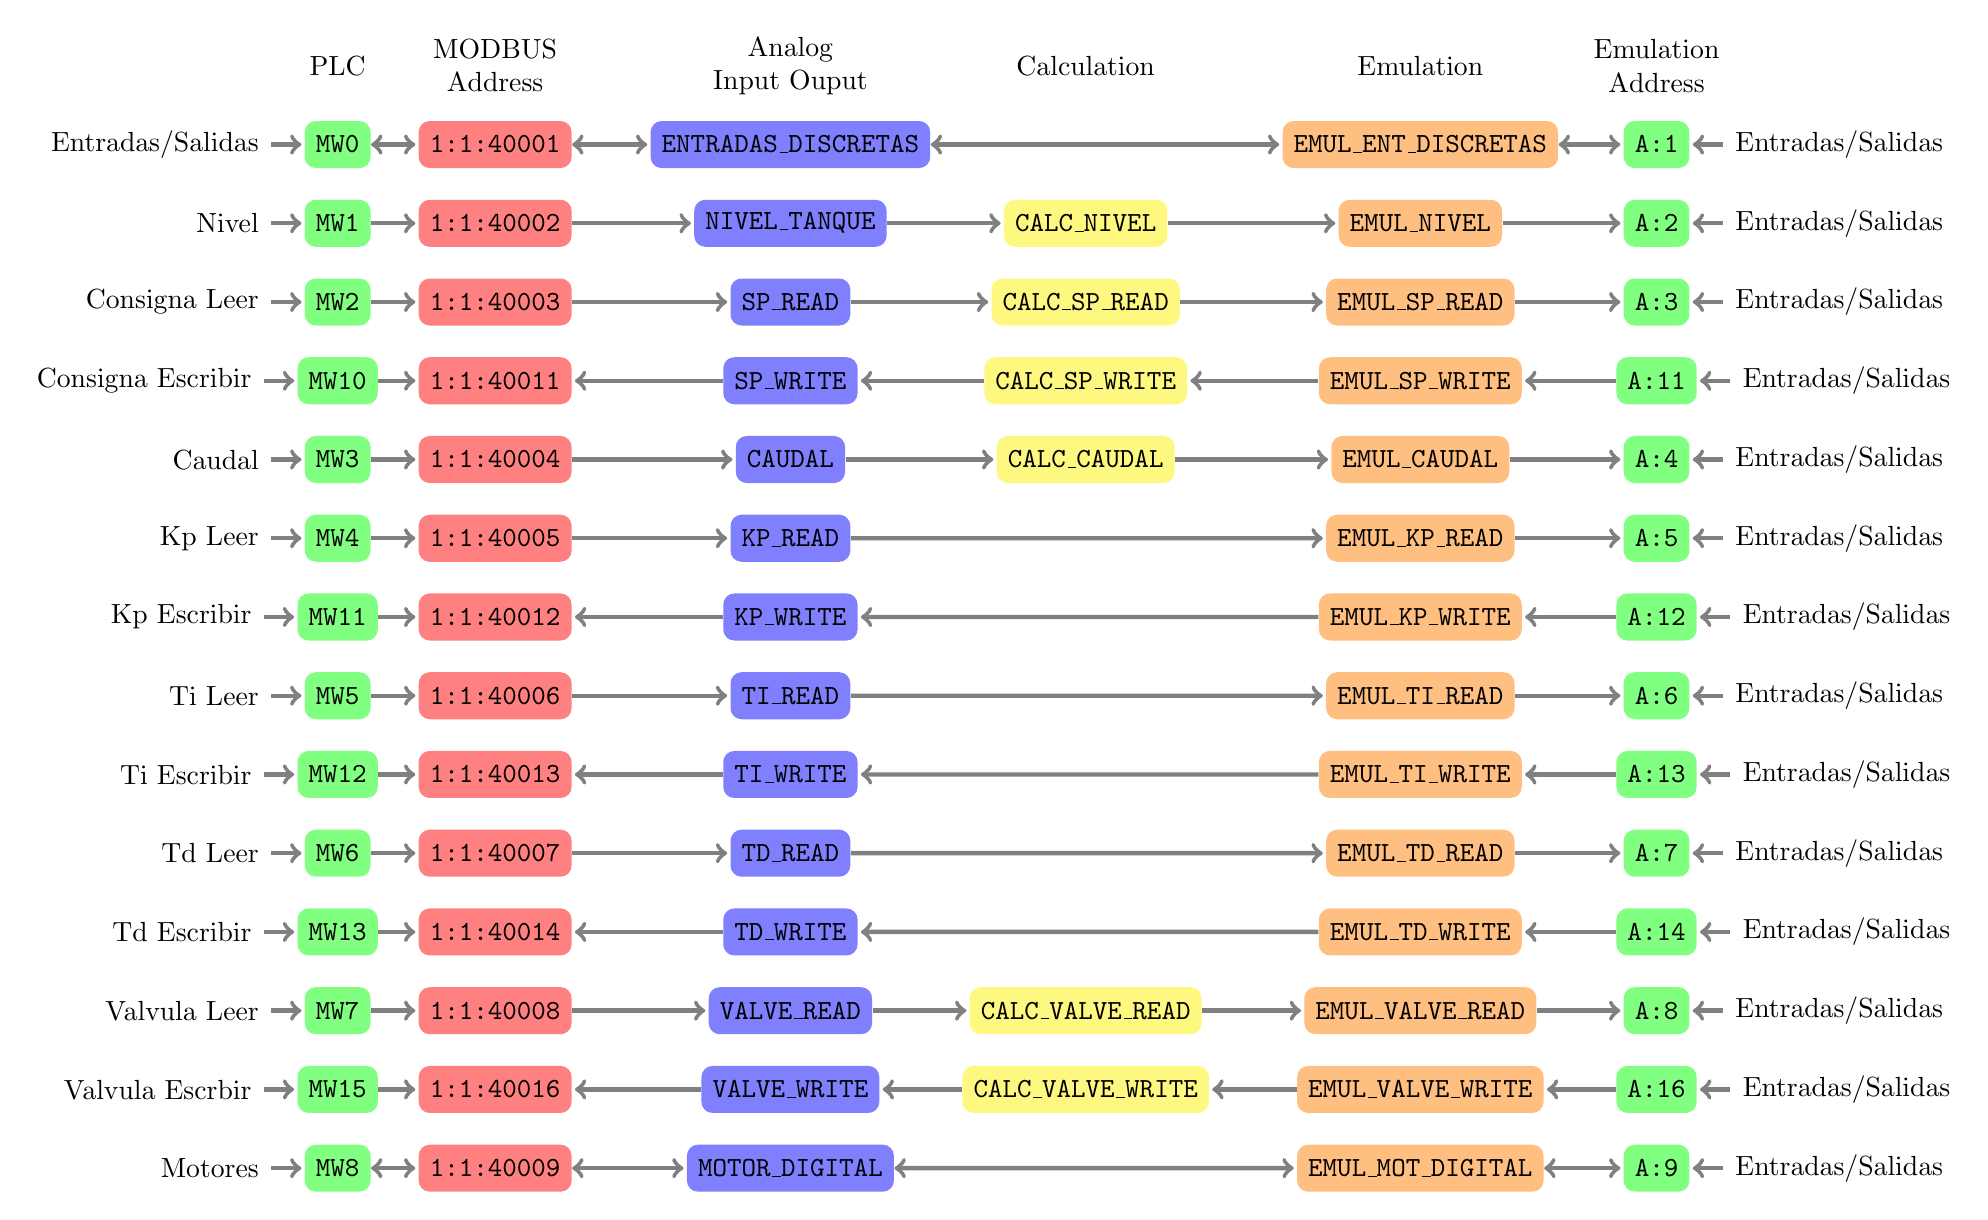
\begin{tikzpicture}[shorten >=1pt,->,draw=black!50]
    \tikzstyle{every pin edge}=[<-,shorten <=1pt, ultra thick]
    \tikzstyle{neuron}=[rectangle,fill=black!25,minimum size=17pt,inner 
sep=4pt, rounded corners]
    \tikzstyle{annot} = [text width=7em, text centered]

    \tikzstyle{plc neuron}=[neuron, fill=green!50];
    \tikzstyle{modbus neuron}=[neuron, fill=red!50, node 
    distance=0.4*5cm];
    \tikzstyle{aio neuron}=[neuron, fill=blue!50, node 
    distance=0.75*5cm];
    \tikzstyle{calc neuron}=[neuron, fill=yellow!50, node 
    distance=0.75*5cm];
    \tikzstyle{emul neuron}=[neuron, fill=orange!50, node 
    distance=0.85*5cm];
    \tikzstyle{emula neuron}=[neuron, fill=green!50, node 
    distance=0.6*5cm];

    % Draw the plc layer nodes
     \node[plc neuron, pin=left:Entradas/Salidas] (mw0) at (0,0) 
{\texttt{MW0}};
     \node[plc neuron, pin=left:Nivel] (mw1) at (0,-1) 
{\texttt{MW1}};
     \node[plc neuron, pin=left: Consigna Leer] (mw2) at (0,-2) 
{\texttt{MW2}};
     \node[plc neuron, pin=left: Consigna Escribir] (mw10) at (0,-3) 
{\texttt{MW10}};
     \node[plc neuron, pin=left: Caudal] (mw3) at (0,-4) 
{\texttt{MW3}};
      \node[plc neuron, pin=left: Kp Leer] (mw4) at (0,-5) 
 {\texttt{MW4}};
      \node[plc neuron, pin=left: Kp Escribir] (mw11) at (0,-6) 
 {\texttt{MW11}};
      \node[plc neuron, pin=left: Ti Leer] (mw5) at (0,-7) 
 {\texttt{MW5}};
      \node[plc neuron, pin=left: Ti Escribir] (mw12) at (0,-8) 
 {\texttt{MW12}};
      \node[plc neuron, pin=left: Td Leer] (mw6) at (0,-9) 
 {\texttt{MW6}};
      \node[plc neuron, pin=left: Td Escribir] (mw13) at (0,-10) 
 {\texttt{MW13}};
      \node[plc neuron, pin=left: Valvula Leer] (mw7) at (0,-11) 
 {\texttt{MW7}};
      \node[plc neuron, pin=left: Valvula Escrbir] (mw15) at (0,-12) 
 {\texttt{MW15}};
      \node[plc neuron, pin=left: Motores] (mw8) at (0,-13) 
 {\texttt{MW8}};

    %Draw Modbus layer nodes
    \node[modbus neuron, right of=mw0] (40001)  {\texttt{1:1:40001}};
    \node[modbus neuron, right of=mw1] (40002)  {\texttt{1:1:40002}};
    \node[modbus neuron, right of=mw2] (40003)  {\texttt{1:1:40003}};
    \node[modbus neuron, right of=mw3] (40004)  {\texttt{1:1:40004}};
    \node[modbus neuron, right of=mw4] (40005)  {\texttt{1:1:40005}};
    \node[modbus neuron, right of=mw5] (40006)  {\texttt{1:1:40006}};
    \node[modbus neuron, right of=mw6] (40007)  {\texttt{1:1:40007}};
    \node[modbus neuron, right of=mw7] (40008)  {\texttt{1:1:40008}};
    \node[modbus neuron, right of=mw8] (40009)  {\texttt{1:1:40009}};
    \node[modbus neuron, right of=mw10] (40011)  {\texttt{1:1:40011}};
    \node[modbus neuron, right of=mw11] (40012)  {\texttt{1:1:40012}};
    \node[modbus neuron, right of=mw12] (40013)  {\texttt{1:1:40013}};
    \node[modbus neuron, right of=mw13] (40014)  {\texttt{1:1:40014}};
    \node[modbus neuron, right of=mw15] (40016)  {\texttt{1:1:40016}};
     
    %Draw Analog Input Output layer nodes
    \node[aio neuron, right of=40001] (io)  {\texttt{ENTRADAS\_DISCRETAS}};
    \node[aio neuron, right of=40002] (niv)  {\texttt{NIVEL\_TANQUE}};
    \node[aio neuron, right of=40003] (spr)  {\texttt{SP\_READ}};
    \node[aio neuron, right of=40004] (caudal)  {\texttt{CAUDAL}};
    \node[aio neuron, right of=40005] (kpr)  {\texttt{KP\_READ}};
    \node[aio neuron, right of=40006] (tir)  {\texttt{TI\_READ}};
    \node[aio neuron, right of=40007] (tdr)  {\texttt{TD\_READ}};
    \node[aio neuron, right of=40008] (vr)  {\texttt{VALVE\_READ}};
    \node[aio neuron, right of=40009] (md)  {\texttt{MOTOR\_DIGITAL}};
    \node[aio neuron, right of=40011] (spw)  {\texttt{SP\_WRITE}};
    \node[aio neuron, right of=40012] (kpw)  {\texttt{KP\_WRITE}};
    \node[aio neuron, right of=40013] (tiw)  {\texttt{TI\_WRITE}};
    \node[aio neuron, right of=40014] (tdw) {\texttt{TD\_WRITE}};
    \node[aio neuron, right of=40016] (vw)  {\texttt{VALVE\_WRITE}};

    %Draw Calculation
    \node[calc neuron, right of=niv] (cniv) {\texttt{CALC\_NIVEL}};
    \node[calc neuron, right of=spr] (cspr) {\texttt{CALC\_SP\_READ}};
    \node[calc neuron, right of=spw] (cspw) {\texttt{CALC\_SP\_WRITE}};
    \node[calc neuron, right of=caudal] (ccaudal) {\texttt{CALC\_CAUDAL}};
    \node[calc neuron, right of=vr] (cvr) {\texttt{CALC\_VALVE\_READ}};
    \node[calc neuron, right of=vw] (cvw) {\texttt{CALC\_VALVE\_WRITE}};
    
    %Draw ResultCalculation
    \node[emul neuron, right of=cniv] (eniv) {\texttt{EMUL\_NIVEL}};
    \node[emul neuron, right of=cspr] (espr) {\texttt{EMUL\_SP\_READ}};
    \node[emul neuron, right of=cspw] (espw) {\texttt{EMUL\_SP\_WRITE}};
    \node[emul neuron, right of=ccaudal] (ecaudal) {\texttt{EMUL\_CAUDAL}};
    \node[emul neuron, right of=cvr] (evr) {\texttt{EMUL\_VALVE\_READ}};
    \node[emul neuron, right of=cvw] (evw) {\texttt{EMUL\_VALVE\_WRITE}};
    
    %Draw Emulation
    \node[emul neuron] (eio) at (2.75*5cm,0 cm) 
{\texttt{EMUL\_ENT\_DISCRETAS}};
    \node[emul neuron] (ekpr) at (2.75*5cm,-5 cm) 
{\texttt{EMUL\_KP\_READ}};
    \node[emul neuron] (etir) at (2.75*5cm,-7 cm) 
{\texttt{EMUL\_TI\_READ}};
    \node[emul neuron] (etdr) at (2.75*5cm,-9 cm) 
{\texttt{EMUL\_TD\_READ}};
    \node[emul neuron] (emd) at (2.75*5cm,-13 cm) 
{\texttt{EMUL\_MOT\_DIGITAL}};
    \node[emul neuron] (ekpw) at (2.75*5cm,-6 
cm){\texttt{EMUL\_KP\_WRITE}};
    \node[emul neuron] (etiw) at (2.75*5cm,-8 cm) 
{\texttt{EMUL\_TI\_WRITE}};
    \node[emul neuron] (etdw) at (2.75*5cm,-10 cm) 
{\texttt{EMUL\_TD\_WRITE}};

    %Draw internal variables
   \node[emula neuron, pin=right:Entradas/Salidas,right of=eio] (a1) 
  {\texttt{A:1}};
  \node[emula neuron, pin=right:Entradas/Salidas,right of=eniv] (a2) 
  {\texttt{A:2}};
  \node[emula neuron, pin=right:Entradas/Salidas,right of=espr] (a3) 
  {\texttt{A:3}};
  \node[emula neuron, pin=right:Entradas/Salidas,right of=espw] (a11) 
  {\texttt{A:11}};
  \node[emula neuron, pin=right:Entradas/Salidas,right of=ecaudal] (a4) 
  {\texttt{A:4}};
  \node[emula neuron, pin=right:Entradas/Salidas,right of=ekpr] (a5) 
  {\texttt{A:5}};
  \node[emula neuron, pin=right:Entradas/Salidas,right of=ekpw] (a12) 
  {\texttt{A:12}};
  \node[emula neuron, pin=right:Entradas/Salidas,right of=etir] (a6) 
  {\texttt{A:6}};
  \node[emula neuron, pin=right:Entradas/Salidas,right of=etiw] (a13) 
  {\texttt{A:13}};
  \node[emula neuron, pin=right:Entradas/Salidas,right of=etdr] (a7) 
  {\texttt{A:7}};
  \node[emula neuron, pin=right:Entradas/Salidas,right of=etdw] (a14) 
  {\texttt{A:14}};
  \node[emula neuron, pin=right:Entradas/Salidas,right of=evr] (a8) 
  {\texttt{A:8}};
  \node[emula neuron, pin=right:Entradas/Salidas,right of=evw] (a16) 
  {\texttt{A:16}};
  \node[emula neuron, pin=right:Entradas/Salidas,right of=emd] (a9) 
  {\texttt{A:9}};

   
  % Connect every node 
  %PLC -> MODBUS
  \path (mw0) edge[<->,ultra thick] (40001); 
  \path (mw1) edge[ultra thick] (40002); 
  \path (mw2) edge[ultra thick] (40003);
  \path (mw3) edge[ultra thick] (40004); 
  \path (mw4) edge[ultra thick] (40005); 
  \path (mw5) edge[ultra thick] (40006); 
  \path (mw6) edge[ultra thick] (40007); 
  \path (mw7) edge[ultra thick] (40008); 
  \path (mw8) edge[<->,ultra thick] (40009);
  \path (mw10) edge[ultra thick] (40011); 
  \path (mw11) edge[ultra thick] (40012); 
  \path (mw12) edge[ultra thick] (40013);
  \path (mw13) edge[ultra thick] (40014); 
  \path (mw15) edge[ultra thick] (40016); 

  %MODBUS -> Analog IO
  \path (40001) edge[<->,ultra thick] (io); 
  \path (40002) edge[ultra thick] (niv); 
  \path (40003) edge[ultra thick] (spr);
  \path (40004) edge[ultra thick] (caudal);
  \path (40005) edge[ultra thick] (kpr);
  \path (40006) edge[ultra thick] (tir);
  \path (40007) edge[ultra thick] (tdr); 
  \path (40008) edge[ultra thick] (vr);
  \path (40009) edge[<->,ultra thick] (md); 
  \path (spw) edge[ultra thick] (40011); 
  \path (kpw) edge[ultra thick] (40012);
  \path (tiw) edge[ultra thick] (40013); 
  \path (tdw) edge[ultra thick] (40014);
  \path (vw) edge[ultra thick] (40016); 

  %Analog -> Calc
  \path (niv) edge[ultra thick] (cniv);
  \path (spr) edge[ultra thick] (cspr);
  \path (cspw) edge[ultra thick] (spw);
  \path (caudal) edge[ultra thick] (ccaudal);
  \path (vr) edge[ultra thick] (cvr);
  \path (cvw) edge[ultra thick] (vw);

  %Calc -> Emulation
  \path (cniv) edge[ultra thick] (eniv);
  \path (cspr) edge[ultra thick] (espr);
  \path (espw) edge[ultra thick] (cspw);
  \path (ccaudal) edge[ultra thick] (ecaudal);
  \path (cvr) edge[ultra thick] (evr);
  \path (evw) edge[ultra thick] (cvw); 
  
  %Analog IO -> Emulation
  \path (io) edge[<->,ultra thick] (eio);
  \path (kpr) edge[ultra thick] (ekpr);
  \path (ekpw) edge[ultra thick] (kpw);
  \path (tir) edge[ultra thick] (etir);
  \path (etiw) edge[ultra thick] (tiw);
  \path (tdr) edge[ultra thick] (etdr);
  \path (etdw) edge[ultra thick] (tdw);
  \path (md) edge[<->,ultra thick] (emd);

  %Emulation -> Address
  \path (eio) edge[<->,ultra thick] (a1);
  \path (eniv) edge[ultra thick] (a2);
  \path (espr) edge[ultra thick] (a3);
  \path  (a11) edge[ultra thick] (espw);
  \path (ecaudal) edge[ultra thick] (a4);
  \path (ekpr) edge[ultra thick] (a5);
  \path  (a12) edge[ultra thick] (ekpw);
  \path (etir) edge[ultra thick] (a6);
  \path  (a13) edge[ultra thick] (etiw);
  \path (etdr) edge[ultra thick] (a7);
  \path (a14) edge[ultra thick] (etdw);
  \path (evr) edge[ultra thick] (a8);
  \path (a16) edge[ultra thick] (evw);
  \path (emd) edge[<->,ultra thick] (a9);
  

 
  % Annotate the layers
  \node[annot,above of=mw0, node distance=1cm] (plc) {PLC};
  \node[annot,above of=40001, node distance=1cm] (modbus) {MODBUS Address};
  \node[annot,above of=io, node distance=1cm] (aio) {Analog Input Ouput};
  \node[annot,right of=aio, node distance=0.75*5cm] (calc) {Calculation};
  \node[annot,above of=eio, node distance=1cm] (emul) {Emulation};
  \node[annot,above of=a1, node distance=1cm] (emula) {Emulation Address};

\end{tikzpicture}
  }
    \caption{Conexion de bloques de la Base de Datos}
    \label{fig:bloqDB}
\end{figure*}

\subsubsection{Creación de los bloques de la base de datos}
A continuación se muestran los pasos necesarios para la creación de un elemento de la base de datos.
% \begin{enumerate}
%  \item Active P-CIM para Windows utilizando el Startup de P-CIM.
%  \item En el directorio de P-CIM oprima el icono del Editor de la Base de Datos.
%  \item Oprima la tecla Add. El Editor de la Base de Datos despliega la ventana de
%   especificaciones de Valor Analógico.
%  \item Ingrese el nombre y complete los campos que correspondan en cada 
% bloque. No se han utilizado
%  el resto de las opciones que presenta la base de datos excepto aquellos que fueron expresados anteriormente 
%  en la tabla \todo{agregar tabla}
%  \item Oprima la tecla OK para regresar al directorio del Bloque.
%  \item Oprima la tecla Save DB para guardar la Base de Datos.
% \end{enumerate}
\begin{table}[H]
\centering
\renewcommand*{\arraystretch}{0.01}
\begin{tabular}{*{2}{m{0.45\textwidth}}}
\hline
  Active P-CIM utilizando el Startup de P-CIM. En el sub-directorio Development 
  de P-CIM oprima el icono del Editor de la Base de Datos
  &\begin{center}
    \rule{0.4\textwidth}{0.3\textwidth}
  \end{center}\\
\hline
  Oprima la tecla Add. El Editor de la Base de Datos despliega la ventana de
  especificaciones de Valor Analógico. Ingrese el nombre y complete los campos 
  que correspondan en cada bloque. No se han utilizado el resto de las opciones 
  que presenta la base de datos excepto aquellos que fueron expresados 
  anteriormente 
  &\begin{center}
    \rule{0.4\textwidth}{0.3\textwidth}
  \end{center}\\
\hline
    Oprima la tecla OK para regresar al directorio del Bloque.
    Oprima la tecla Save DB para guardar la Base de Datos.
  &\begin{center}
    \rule{0.4\textwidth}{0.3\textwidth}
  \end{center}\\
\hline
\end{tabular}
\label{tab:confBlockDB}
\caption{Configuración de los bloques de la base de datos.}
\end{table}



Ahora podemos controlar el funcionamiento del bloque recién configurado de la 
siguiente manera:
\begin{enumerate}
  \item Abra el Datascope (Monitor de Datos), con un doble click sobre su icono 
  en el directorio de P-CIM.
  \item Escriba el nombre de alguno de los bloques antes definidos  y en otro 
  item su dirección.
  \item Se debe poder observar en ambos el mismo valor leído(en caso de 
  registros de lectura) o el mismo valor al escribir en uno u otro de los items.
\end{enumerate}
Si esta prueba nos ha dado los resultados esperados podemos estar seguros que 
nuestros bloques se encuentran bien configurados y podemos proseguir con el 
desarrollo de nuestro sistema \gls{scada}.


\subsection{Capa de aplicación}
\label{subsec:CapaAplicacion}
La tercer y última capa del sistema \gls{scada} es la capa de aplicación. Esta 
será utilizada en nuestro \gls{pfe} unicamente como \gls{hmi}. Para el 
desarrollo de la interfaz gráfica definimos un documento gráfico creado con el 
Editor de Animaciones (Animation Editor). Finalmente, mediante el Servidor de 
Pantallas (Operator Workstation) se pone en marcha el sistema. A continuación se 
presentan el desarrollo y descripción de la pantalla realizada mediante las 
herramientas gráficas provistas por P-CIM.

%Incluye ilustraciones, indicadores y controles emulando un panel de control 
%real pero con muchos más elementos. Actúa como interfase entre el operador y 
%la planta.


\subsubsection{Diseño de una pantalla}
El primer paso en el diseño de un pantalla es la definición de requerimientos 
con los que debemos cumplir. Estos se resumen en:
\begin{itemize}
 \item Botones de encendido y parada de la planta.
 \item Visualización del estado actual de la planta: Niveles, caudal, bombas 
 encendidas, etc.
 \item Control Manual
 \begin{itemize}
  \item Encender las bombas de manera independiente.
  \item Controlar la abertura de la válvula
 \end{itemize}
 \item Control Automático
 \begin{itemize}
  \item Visualizar el seguimiento de la consigna.
  \item Visualizar/Definir la consigna
  \item Visualizar/Definir las constantes del controlador
 \end{itemize}
\end{itemize}

Ahora mediante el Editor de Animaciones (ubicado en el sub-directorio 
Development) diseñaños y definimos las características funcionales de 
la pantalla que correrá en el Operator Workstation. Mediante las 
características antes especificadas se obtuvo el resultado que se observa en la 
figura \todo{agregar figura hmi}. 

Para dicha interfaz se procedió en el siguiente orden:
\begin{enumerate}
 \item Iniciar el Editor de Animaciones. Elegir el icono de la carpeta de P-CIM. Aparece un pantalla 
 sin nombre. Guarde el archivo asignandole un nombre.
 \item Crear la ilustración básica.\\
    Use el Editor de Animaciones para  dibujar sus propios gráficos 
    o insertar objetos gráficos ya creados de la biblioteca de ClipArt.Los objetos gráficos insertados 
    desde el ClipArt pueden tratarse como cualquier otro objeto gráfico y ser movidos, redimensionados, 
    editados y asignados con propiedades.
    Para seleccionar un objeto de ClipArt:
    \begin{enumerate}
      \item Elegir "’ClipArt” en el menú File, luego elegir la categoría en el submenú o elegir el botón 
      categoría de la caja de ClipArt.
      \item Hacer click en el objeto para seleccionarlo.
      \item Hacer click nuevamente sobre el objeto seleccionado, mantener presionada la tecla CTRL y 
      el botón izquierdo del mouse, arrastrar el objeto hasta el lugar deseado en el pantalla y soltar 
      el botón del mouse y la tecla CTRL. La ventana de ClipArt se cierra tan pronto Ud. comienza a 
      arrastrar el objeto.
    \end{enumerate}

 \item Animar la ilustración.\\
      Para animar un objeto gráfico se debe seleccionar el objeto y especificar una o
      más propiedades de la Lista de Propiedades (Properties List).
      Para comenzar a animar un objeto
      \begin{enumerate}
	\item Seleccionar el objeto (click izquierdo del mouse); por ejemplo un rectángulo. El
	Editor de Animaciones le coloca marcas al objeto.
	\item Elegir Properties List (Lista de Propiedades) 
      \end{enumerate}
      Las propiedades están divididas en tres
      categorías principales: Controls, Indicators y Special 
      (controles, indicadores y especiales).
      \begin{itemize}
	\item  Controls: especifica una entrada de datos la cual puede estar dada por 
	casillas de entrada de datos, botones que inician acciones, o
	potenciómetros que permiten fijar valores analógicos.
	\item Indicators: Usados para crear presentaciones textuales, de color
	y gráficas de los datos, en estos los contenidos, posición, color y
	tamaño cambian en función del valor de los datos.
	\item Special: esta categoría es usada para especificar Gráficos de Tendencia o
	“Medidores de Desviación”.
      \end{itemize}
      Un signo de visto en una casilla de propiedades significa que ésta es la propiedad
      asignada al objeto gráfico. Luego aparece otra ventana de diálogo:
      donde se debe completar (Servidor, Tópico e Item) para cada
      propiedad que especifique (excepto para el botón). Esto designa
      respectivamente el origen de los datos mostrados por el indicador o 
      el destino de los datos escritos por el objeto de control.
      
 \item Probar los resultados en el Operator Workstation.\\
      Para poder probar el funcionamiento de nuestra \gls{hmi} procedemos de la siguiente manera:
      \begin{enumerate}
       \item 
      \end{enumerate}
\end{enumerate}
 

\section{Ejecución}
\label{sec:Ejecucion}

Una ves que han sido configuradas cada una de las partes podemos utilizar nuestro sistema SCADA.


\chapter{Conclusiónes}
\label{ch:conclusiones}

\section{Conclusión Técnica}
\label{sec:ConclusionTecnica}
Espero que estemos inspirados a esta altura. \cite{Gardner}


\section{Perspectivas}
\label{sec:Perspectivas}
Y más para acá. \gls{pwm}

\section{Conclusión Personal}
\label{sec:ConclusionPersonal}

Con este proyeto se termina una etapa de nuestras vidas, un
ciclo que culmina y es por ello la importancia que tiene para
nosotros este


%%%%%%%%%%%%%%%%%%%%%%%%%%%%%%%%%%%%%%%%%%%%%%%%%%%%%%%%%%%%%%%%%%%%%%%%
%%------------------------------%%
%%            		  	%%
%%   GLOSARIO Y BIBLIOGRAFIA	%%
%%            			%%
%%------------------------------%%
\backmatter


\setlength{\glslistdottedwidth}{0.4\textwidth}
\setglossarystyle{listdotted} % mirror.ox.ac.uk/sites/ctan.org/macros/latex/contrib/glossaries/glossaries-user.html#dx1-35001
\printglossaries
\bibliographystyle{ieeetr}
\bibliography{Bibliografia/bibliografia}
\addcontentsline{toc}{chapter}{Bibliografía}

\appendix
\chapter{Anexos}
\section{Este es un ejemplo de anexo}
\label{anexo:Ejemplo}

\cleardoublepage


\end{document}
